\RequirePackage{fix-cm}
\documentclass[smallextended]{svjour3}
\smartqed

\usepackage[utf8]{inputenc}
\usepackage{amsmath, amssymb, amsfonts}
\usepackage{graphicx}
\usepackage{array}
\usepackage{tikz}
\usetikzlibrary{shapes.geometric, arrows, positioning, decorations.pathreplacing, fit, backgrounds}
\usepackage{booktabs}
\usepackage{microtype}
\usepackage[hidelinks]{hyperref}
\usepackage{orcidlink}
\usepackage{makecell}
\usepackage{adjustbox}
% Render bibliography DOIs as full DOI links, as the journal requires.
\providecommand{\doi}{}
\renewcommand{\doi}[1]{\href{https://doi.org/#1}{https://doi.org/#1}}
\usepackage[numbers,sort&compress]{natbib}
\usepackage{float}

\begin{document}
\sloppy

\title{Continuous-state robust CVaR portfolio optimization via grid-restricted constraint generation}
\titlerunning{Continuous-state robust CVaR portfolio optimization}

\author{Madani Bezoui \and Thiziri Sifaoui \and Ahcene Bounceur}
\authorrunning{M. Bezoui \and T. Sifaoui \and A. Bounceur}

\institute{Madani Bezoui (corresponding author) \at
              CESI LINEACT, UR 7527, Nancy, France \\
              \email{mbezoui@cesi.fr} --- ORCID \orcidlink{0000-0002-8342-7039}~0000-0002-8342-7039
           \and
           Thiziri Sifaoui \at
              Department of Mathematics and Computer Science, University of Amine Elokkal El Hadj Moussa Eg Akhamouk, Tamanghasset, Algeria \\
              LAROMAD, Faculty of Sciences, UMMTO, Tizi Ouzou, Algeria --- ORCID \orcidlink{0009-0007-6884-0611}~0009-0007-6884-0611
           \and
           Ahcene Bounceur \at
              College of Computing and Informatics, University of Sharjah, United Arab Emirates --- \email{abounceur@sharjah.ac.ae} --- ORCID \orcidlink{0000-0002-0043-7742}~0000-0002-0043-7742
}

\date{}

\maketitle

\begin{abstract}
Standard robust portfolio optimization models represent market conditions through discrete regimes or unconditional ambiguity sets. We instead formulate a continuous-state robust portfolio model that minimizes Conditional Value-at-Risk (CVaR) uniformly over a continuously indexed family of kernel-weighted empirical conditional return distributions, with states indexed by the logarithm of the CBOE Volatility Index (log-VIX) and market drawdown. We establish well-posedness, continuity and convexity of the continuous formulation and derive a Lipschitz bound on the grid-discretization error. For computation we employ a grid-restricted separation oracle and solve the finite approximation by adaptive constraint generation, which on a representative instance cuts the master problem from 441 to 5 state blocks and the solve time from 72.7 to 4.5 seconds. In a rolling out-of-sample study of US industry portfolios, 1994--2026, the strategy achieves competitive long-run wealth, but a paired circular moving-block percentile bootstrap provides no evidence of a statistically significant Sharpe-ratio advantage over nominal CVaR. The findings highlight the importance of data support in tail regions and establish the tractability of a grid-restricted approximation to continuous-state robustification.
\keywords{Robust Portfolio Optimization \and Conditional Value-at-Risk \and Semi-Infinite Programming \and Kernel-Weighted Conditional Distributions \and Constraint Generation}
\end{abstract}

\section{Introduction}
The classical mean-variance framework introduced by \cite{markowitz1952portfolio} established the quantitative foundation of modern portfolio theory. However, the practical implementation of mean-variance optimization has long been hindered by its extreme sensitivity to parameter estimation errors. Small perturbations in expected returns or covariance estimates often produce erratic allocations, excessive portfolio turnover, and severe out-of-sample disappointment. To address these vulnerabilities, researchers have developed robust portfolio optimization techniques that optimize allocations against the worst-case parameters within prespecified uncertainty sets \cite{goldfarb2003robust, fabozzi2007robust}. Concurrently, various exact, iterative, and metaheuristic methods have been developed to handle complex real-world constraints in portfolio selection \cite{bezoui2019iterative, regaigui2025memetic}, as well as in broader multi-objective manufacturing and supply chain contexts \cite{bezoui2024hybrid}.

Traditional robust portfolio models predominantly focus on unconditional uncertainty sets constructed around historical sample moments or empirical distributions \cite{delage2010distributionally, esfahani2018data}. While these models effectively mitigate sensitivity to estimation noise, they typically treat market dynamics as stationary and homogeneous across time. In reality, financial markets exhibit pronounced state-dependent behavior. During tranquil market environments, asset correlations remain moderate and return dispersions offer meaningful diversification benefits. In contrast, during periods of acute financial distress, volatility spikes, asset correlations tend to increase, and tail risks materialize simultaneously across sectors.

To incorporate state dependence, a common practice in financial econometrics is to employ discrete regime-switching models \cite{ang2002international}. These models segment market history into a small, finite collection of latent states, such as low-volatility expansionary regimes and high-volatility contractionary regimes. While finite regime classifications offer conceptual simplicity and computational tractability, they impose a discretization on market dynamics. Often, market stress evolves along a continuous spectrum of financial-market conditions. An abrupt jump between two discrete regimes may fail to capture intermediate stress levels and boundary dynamics where vulnerability to systemic shocks varies more continuously.


In this context, our work investigates how a continuous-state robust formulation compares structurally and empirically to standard unconditional and discrete-regime robust portfolio models. We explore whether adaptive constraint generation can effectively scale continuous-state portfolio robustification to overcome the computational limits of dense enumeration. Furthermore, we examine whether state-domain continuous robustification improves out-of-sample risk-adjusted returns and downside protection across non-stationary market environments, and we analyze the role of model regularization---such as bandwidth scaling and empirical support thresholding---in mitigating boundary scenario overfitting within continuous robust sets.

In this paper, we propose a continuous-state robust portfolio optimization framework that bridges non-parametric conditional risk modeling and semi-infinite optimization. Rather than partitioning market history into discrete regimes, we define a continuous, compact state space $\mathcal{U} \subset \mathbb{R}^2$ spanned by observable financial indicators: the logarithm of the CBOE Volatility Index (log-VIX) \cite{cboe2026vix} and the trailing equity market drawdown. Every point $\theta \in \mathcal{U}$ represents a distinct market environment and induces a well-defined conditional empirical return distribution constructed via multivariate Nadaraya--Watson kernel weighting \cite{nadaraya1964estimating, watson1964smooth}.

The investor seeks an allocation that minimizes the worst-case Conditional Value-at-Risk (CVaR) over the entire continuous state space $\mathcal{U}$:
\begin{equation}
    \min_{w \in W} \max_{\theta \in \mathcal{U}} \Phi_\tau(w, \theta)
\end{equation}
where $W$ is the capped portfolio simplex and $\Phi_\tau(w, \theta)$ is the conditional CVaR at confidence level $1-\tau = 0.95$ under the empirical measure induced by state $\theta$. We emphasize that this model is a \emph{state-robust} portfolio model, not distributionally robust optimization. For each state $\theta$, the conditional distribution is fixed by the kernel weights, and no distributional ambiguity set is placed around that conditional distribution. Furthermore, the term ``adaptive'' in our framework refers specifically to \emph{adaptive constraint generation} via a semi-infinite exchange algorithm, rather than a decision policy $w(y_t)$ dynamically conditioned on the current state. The optimal allocation $w$ immunizes against all states in $\mathcal{U}$, while dynamic reallocation over time results from rolling-window re-estimation of the return-state relationship.

Because the state space $\mathcal{U}$ is uncountable, this formulation gives rise to a Semi-Infinite Program (SIP) with an infinite collection of joint risk constraints. Direct solution via dense spatial discretization becomes computationally prohibitive and scales poorly in high dimensions. To solve a finite grid-restricted approximation of the continuous-state SIP efficiently, we use an adaptive exchange algorithm. The method alternates between solving a finite master linear program over a sparse active subset of grid states and executing a full-grid separation oracle that identifies the most adverse state on the candidate grid for the current portfolio.

Our primary contribution is methodological and empirical: We formulate a state-robust portfolio model that minimizes CVaR uniformly over a continuously indexed family of kernel-weighted empirical conditional return distributions. We establish basic well-posedness and convexity properties of the continuous formulation. For computation, we solve a finite grid-restricted approximation using constraint generation, which substantially reduces master-LP size relative to dense enumeration. A multi-decade out-of-sample study shows competitive wealth but no statistically significant Sharpe-ratio advantage over simpler benchmarks, while highlighting the importance of data support at adversarial market states.

To facilitate open science, reproducibility and independent verification of all empirical findings, the complete Julia and Python codebase, the cleaned financial datasets, and all figure generation routines are maintained in an open-source repository \cite{bezoui2026robust}.

The remainder of this manuscript is structured as follows. Section \ref{sec:related} reviews related literature across robust optimization, conditional stochastic programming, and semi-infinite algorithms. Sections \ref{sec:model} and \ref{sec:theory} develop the continuous-state modeling framework, kernel weighting mechanics, and theoretical existence theorems. Section \ref{sec:algorithms} presents the adaptive exchange algorithm and distinguishes exact continuous separation from the grid-restricted separation used in the numerical implementation. Section \ref{sec:experimental} details the rolling-window backtesting protocol, while Sections \ref{sec:results} and \ref{sec:computational} report empirical and computational results across approximately 31.5 years. Section \ref{sec:sensitivity} presents model-specification sensitivity analysis, and Section \ref{sec:conclusion} provides discussion, practical limitations, and concluding remarks.

\section{Related work}\label{sec:related}
Our methodology intersects three active streams of quantitative operations research: robust portfolio selection, conditional stochastic programming with side information, and semi-infinite optimization algorithms.

\subsection{Classical and distributionally robust portfolio selection}
Classical robust portfolio selection addresses the sensitivity of Markowitz mean-variance optimization to estimation noise by assuming that expected return vectors and covariance matrices reside in deterministic uncertainty sets \cite{goldfarb2003robust, fabozzi2007robust}. Concurrently, various exact, iterative, and metaheuristic methods have been developed to handle complex real-world constraints in portfolio selection \cite{bezoui2019iterative, regaigui2025memetic}, as well as in broader multi-objective manufacturing and supply chain contexts \cite{bezoui2024hybrid}. These formulations yield second-order cone or semidefinite programs that provide worst-case guarantees. However, moment-based robust models frequently rely on implicit symmetry assumptions that fail to reflect the severe skewness, heavy tails, and asymmetric dependence structures inherent in financial return distributions.

To capture tail risk directly, \cite{rockafellar2000optimization, rockafellar2002conditional} introduced the Conditional Value-at-Risk (CVaR) as a coherent risk measure that can be optimized efficiently via linear programming. Building on this foundation, distributionally robust optimization (DRO) seeks to minimize risk over an ambiguity set of probability distributions constructed around an empirical baseline. Modern DRO frameworks define ambiguity balls using moment constraints \cite{delage2010distributionally} or optimal transport metrics such as the Wasserstein distance \cite{esfahani2018data}.

Recent theoretical developments in DRO have expanded its algorithmic scope. For instance, \cite{chu2025wasserstein} propose tractable regularized reformulations of Wasserstein DRO problems that achieve global convergence, while \cite{agra2025two} analyzes two-stage distributionally robust programs with finite supports. In related structural contexts, \cite{yue2026geometric} draw geometric connections between ambiguity sets and covariance shrinkage, and \cite{thoma2026piecewise} study piecewise affine decision rules for robust multi-stage settings.

\subsection{Conditional stochastic optimization and covariate side information}
A rapidly expanding body of literature investigates how observable side information (covariates) can be integrated into data-driven decision-making. \cite{bertsimas2020predictive} established a general framework for predictive prescriptions, demonstrating that non-parametric kernel regression, $k$-nearest neighbors, and tree-based weights can effectively condition decision problems on prevailing covariates. In the context of risk management, \cite{scaillet2004nonparametric} examined non-parametric kernel estimation of conditional expected shortfall.

In recent contributions, \cite{qi2026integrated} introduce an integrated conditional estimation-optimization methodology that directly couples regression trees with downstream optimization tasks, minimizing decision error rather than prediction loss. \cite{bennouna2025learning} explore phase transitions in data-driven decision-making, providing optimal sample complexity bounds for prescriptive models with side information. Earlier foundational frameworks in conditional DRO include \cite{esteban2022distributionally}, who developed distributionally robust stochastic programs with side information based on trimmed Wasserstein balls, and \cite{nguyen2025robustifying}, who formulated robust conditional portfolio decisions via optimal transport metrics centered on covariate-conditioned empirical distributions.

Closest in spirit to the present computational setting, \cite{chenreddy2022conditional} learn contextual uncertainty sets and solve the resulting conditional robust programs by constraint generation; their sets are learned around the observed context, whereas the family indexed here is fixed by the kernel construction and the robustness is taken over the whole state domain rather than around one observed state.

Our framework differs in its mathematical construction from conditional DRO. In conditional DRO, the decision-maker constructs an ambiguity set around the conditional distribution corresponding to the currently observed state $y_t$. In our continuous-state robust model, we do not restrict attention to a single observed state. Instead, we seek an allocation that remains robust across the entire family of kernel-weighted conditional distributions induced by all states $\theta \in \mathcal{U}$. We refer to this approach as continuous-state robust optimization over kernel-weighted empirical conditional distributions.


To distinguish our approach from standard Conditional Distributionally Robust Optimization (DRO), consider the formal structures:
\begin{align}
\text{Conditional DRO:} &\quad \min_{w \in W}\;\sup_{P \in \mathcal{B}(\hat{P}_{y_t})}\; \mathrm{CVaR}_{P}(w) \label{eq:dro_contrast} \\
\text{This paper (Robust SIP):} &\quad \min_{w \in W}\;\sup_{\theta \in \mathcal{U}}\; \mathrm{CVaR}_{\hat{P}_\theta}(w) \label{eq:sip_contrast}
\end{align}
The robustification operator differs significantly: standard DRO considers a measure-ball $\mathcal{B}$ around a fixed covariate $y_t$, whereas we take a supremum over a covariate-indexed family of fixed empirical measures over a continuous state space $\mathcal{U}$. Consequently, the optimization structure differs (single-state DRO reformulations versus SIP with a continuum of LP blocks). These approaches are complementary, and one could in principle compose them in future work.

\subsection{Semi-infinite programming and exchange algorithms}
Semi-infinite programming (SIP) considers optimization problems with a finite number of decision variables and an infinite index set of constraints \cite{hettich1993semi, lopez2007semi}. SIP techniques have found applications in engineering design, robust control, and spectral estimation, but their operational use in financial portfolio allocation has been constrained by computational complexity.

The standard solution paradigm for convex SIPs is the cutting-plane or exchange algorithm. At each iteration, the master problem solves a relaxed subproblem over a finite subset of constraints, while a separation oracle identifies the most violated constraint across the continuous index set. When the oracle can be solved to certified global optimality, the exchange algorithm generates monotonically non-decreasing lower bounds and certified upper bounds that converge to the true global optimum. In practical settings where the oracle is solved over a grid or via local search heuristics, exact continuous separation is relaxed. For broader methodological context, \cite{oustry2025convex} formalize the convergence and error propagation of convex SIP algorithms equipped with inexact separation oracles.


Table \ref{tab:lit_comparison} positions the present framework relative to these
strands of the literature, contrasting for each model family the information
used to index the market state, the way the conditional distribution is
represented, whether the resulting decision is state-dependent, the dimension
along which robustness is imposed, and the computational form that must
ultimately be solved. In the table, weighted SAA denotes weighted sample
average approximation.

\begin{table}[htbp]
\centering
\caption{Comparison of conditional and robust risk models}
\label{tab:lit_comparison}
\begin{tabular}{>{\raggedright\arraybackslash}p{0.18\linewidth}>{\raggedright\arraybackslash}p{0.17\linewidth}>{\raggedright\arraybackslash}p{0.26\linewidth}>{\raggedright\arraybackslash}p{0.24\linewidth}}
\toprule
\textbf{Paradigm} & \textbf{Objective} & \textbf{Distributional Assumption} & \textbf{Covariate Role} \\
\midrule
Unconditional Markowitz & Mean-Variance & Stationary Gaussian & None \\
Nominal Conditional & Expected Shortfall & True conditional $P(Y \mid X)$ known & Directly defines the distribution \\
Standard DRO & Worst-case Risk over $\mathcal{P}$ & Global ambiguity set $\mathcal{P}$ & Typically unconditional \\
Covariate-driven DRO & Conditional Worst-case Risk & State-dependent ambiguity set $\mathcal{P}(x)$ & Centers the conditional ambiguity set \\
\textbf{Robust SIP (Proposed)} & \textbf{Worst-case Risk over $\mathcal{U}$} & \textbf{Continuous kernel-weighted empirical} & \textbf{Defines a continuous geometric state space $\mathcal{U}$} \\
\bottomrule
\end{tabular}
\end{table}




\section{Model}\label{sec:model}
We consider an investment universe consisting of $N$ risky financial assets over a discrete time horizon $t = 1, \dots, T$. Let $x_t = (x_{1,t}, \dots, x_{N,t})^\top \in \mathbb{R}^N$ denote the vector of realized asset returns from trading day $t-1$ to day $t$. The joint conditional distribution of asset returns is modulated by prevailing financial-market state variables observable at time $t-1$, denoted by the vector $y_{t-1} \in \mathbb{R}^M$.

\subsection{State variable selection and compact state space}
In this study, we focus on two primary financial indicators that capture distinct dimensions of market risk ($M = 2$): the logarithm of the CBOE Volatility Index, $\log V_t$ (log-VIX), and the Trailing Market Drawdown ($D_t$) representing the peak-to-trough decline of the broad equity market index over a trailing quarterly lookback window of $L = 63$ trading days:
\begin{equation}
    D_t = 1 - \frac{P_t}{\max_{s \in [t-L, t]} P_s} \in [0, 1]
\end{equation}
where $P_t$ is the cumulative total return index of the broad market proxy (computed as the equal-weighted composite of the 30 industry portfolios). The choice of an equal-weighted proxy rather than a value-weighted aggregate is deliberate: the equal-weighted index is more sensitive to distress in smaller sectors and therefore serves as a more responsive indicator of broad-based distress across the entire opportunity set. By construction, $D_t \ge 0$ measures positive drawdown severity ($0\%$ representing peak wealth, and positive values indicating drawdown depth).

The state vector at time $t-1$ is $y_{t-1} = (\log V_{t-1}, D_{t-1})^\top \in \mathbb{R}^2$. For each rolling training window, define
\begin{equation}
v_{\min}=\min_t \log V_{t-1},\qquad v_{\max}=\max_t \log V_{t-1},
\end{equation}
and
\begin{equation}
d_{\min}=\min_t D_{t-1},\qquad d_{\max}=\max_t D_{t-1}.
\end{equation}
All extrema, variances, bandwidths, and grid boundaries are recomputed exclusively from the current 1,260-day training window. We define the continuous state space $\mathcal{U} \subset \mathbb{R}^2$ as a compact rectangle containing all historically observed market states, augmented by a fixed 10\% outer margin to examine states slightly beyond the observed training-window extrema, while strictly respecting the non-negative domain of drawdown:
\begin{equation}
    \mathcal{U} = [v_{\min} - \delta_v, v_{\max} + \delta_v] \times [\max\{0, d_{\min} - \delta_d\}, \min\{1, d_{\max} + \delta_d\}]
\end{equation}
where $\delta_v = 0.10 (v_{\max} - v_{\min})$ and $\delta_d = 0.10 (d_{\max} - d_{\min})$. The lower bound on drawdown is clamped at 0, preventing negative drawdown values. By construction, $\mathcal{U}$ is a closed and bounded subset of $\mathbb{R}^2$, ensuring compactness.

\begin{remark}[Domain rectangularity and empirical support]
The Cartesian bounding box $\mathcal{U}$ treats every combination of VIX and drawdown as plausible. However, certain corners (e.g., very high VIX with zero drawdown) have low empirical support. In our empirical analysis, we track the Effective Sample Size of active states to monitor local data support, and we evaluate regularized uncertainty sets $\mathcal{U}_{\text{supp}} = \{\theta \in \mathcal{U} : \operatorname{ESS}(\theta) \ge E_{\min}\}$ in Section \ref{sec:sensitivity}.
\end{remark}






\subsection{Kernel-weighted conditional distributions and effective sample size}
For any continuous state query $\theta = (v_\theta, d_\theta)^\top \in \mathcal{U}$, we construct a state-dependent empirical probability distribution over historical return realizations $\{x_1, \dots, x_T\}$. Each historical return observation $x_t$ is assigned a Nadaraya--Watson kernel weight \cite{nadaraya1964estimating, watson1964smooth} based on the proximity of its preceding state $y_{t-1}$ to the target state $\theta$:
\begin{equation}
    p_t(\theta) = \frac{K_H(y_{t-1} - \theta)}{\sum_{s=1}^{T} K_H(y_{s-1} - \theta)} = \frac{\exp\left(-\frac{1}{2}(y_{t-1} - \theta)^\top H^{-1} (y_{t-1} - \theta)\right)}{\sum_{s=1}^T \exp\left(-\frac{1}{2}(y_{s-1} - \theta)^\top H^{-1} (y_{s-1} - \theta)\right)}
\end{equation}
where $H \in \mathbb{R}^{2 \times 2}$ is a symmetric positive-definite bandwidth matrix. We specify $H$ using the bivariate rule-of-thumb \cite{silverman1986density}, defined by marginal bandwidths $h_m = T^{-1/6}\hat\sigma_m$:
\begin{equation}
    H = \operatorname{diag}\left(h_{\text{log-VIX}}^2, h_{\text{DD}}^2\right) = T^{-1/3} \operatorname{diag}\left(\hat{\sigma}_{\text{log-VIX}}^2, \hat{\sigma}_{\text{DD}}^2\right)
\end{equation}
for $M = 2$, where $\hat{\sigma}^2_{\log\text{-VIX}}$ and $\hat{\sigma}^2_{\text{DD}}$ are the sample variances of log-VIX and drawdown, respectively, computed over the current training window. The diagonal bandwidth matrix scales the two state dimensions by their respective sample variances but does not account for their empirical cross-covariance. While log-VIX and drawdown exhibit non-trivial empirical correlation, using a diagonal matrix acts as a form of geometric regularization that avoids excessively narrow, elongated kernel contours that could overfit the historical dependence structure. Future work could explore full-covariance bandwidth selection methods to further refine the shape of the conditional empirical measure.

Because the Gaussian kernel is strictly positive everywhere on $\mathbb{R}^2$, the normalization denominator is strictly positive for all $\theta \in \mathcal{U}$. Consequently, the kernel weights satisfy $p_t(\theta) > 0$ and $\sum_{t=1}^T p_t(\theta) = 1$ for every $\theta \in \mathcal{U}$. Each continuous state $\theta$ induces a well-defined conditional empirical distribution $\mathbb{P}(X | \theta) = \sum_{t=1}^{T} p_t(\theta) \delta_{x_t}$ (as illustrated in Figure \ref{fig:schema1}), where $\delta_{x_t}$ denotes the Dirac delta mass at historical return vector $x_t$.

To monitor local data support across the continuous domain, we compute the Effective Sample Size (ESS) for any state $\theta \in \mathcal{U}$:
\begin{equation}
    \text{ESS}(\theta) = \frac{1}{\sum_{t=1}^T p_t(\theta)^2}
\end{equation}
When weights are uniformly distributed ($p_t(\theta) = 1/T$), the ESS reaches its theoretical maximum $\text{ESS}(\theta) = T$. Conversely, if all weight concentrates on a single historical observation, $\text{ESS}(\theta) = 1$. For descriptive purposes, we report $\tau\times \operatorname{ESS}(\theta)$ as a coarse tail-support proxy. Because kernel weights are non-uniform and tail membership depends on the ordering of portfolio losses, this quantity should not be interpreted as a formal tail effective sample size.

\begin{figure}[htbp]
\centering
\resizebox{0.92\textwidth}{!}{
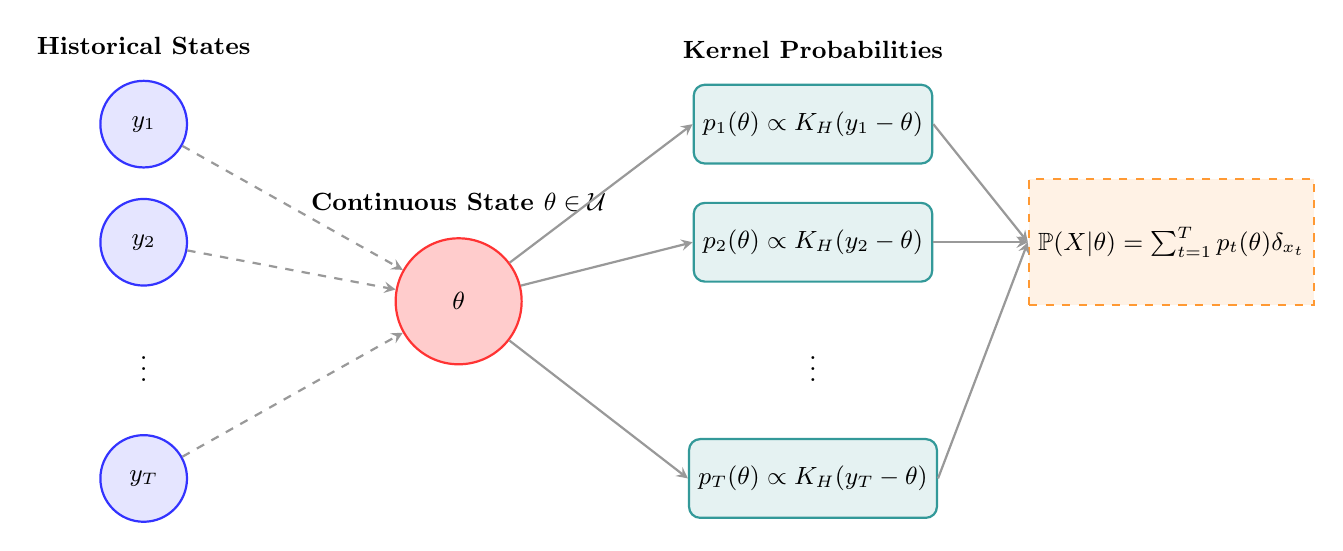
\begin{tikzpicture}[
    node distance=2cm,
    state/.style={circle, draw=blue!80, fill=blue!10, thick, minimum size=1.1cm, font=\small},
    kernel/.style={rectangle, draw=teal!80, fill=teal!10, rounded corners, thick, minimum height=1cm, font=\small},
    dist/.style={rectangle, draw=orange!80, fill=orange!10, dashed, thick, minimum width=3.4cm, minimum height=1.6cm, font=\small},
    arrow/.style={thick, ->, >=stealth, color=gray!80}
]

\node[state] (y1) at (0, 3) {$y_1$};
\node[state] (y2) at (0, 1.5) {$y_2$};
\node at (0, 0) {\vdots};
\node[state] (yT) at (0, -1.5) {$y_T$};

\node[above=0.2cm of y1, font=\bfseries\small] {Historical States};

\node[state, fill=red!20, draw=red!80, minimum size=1.6cm] (theta) at (4, 0.75) {$\theta$};
\node[above=0.2cm of theta, font=\bfseries\small] {Continuous State $\theta \in \mathcal{U}$};

\node[kernel] (k1) at (8.5, 3) {$p_1(\theta) \propto K_H(y_1 - \theta)$};
\node[kernel] (k2) at (8.5, 1.5) {$p_2(\theta) \propto K_H(y_2 - \theta)$};
\node at (8.5, 0) {\vdots};
\node[kernel] (kT) at (8.5, -1.5) {$p_T(\theta) \propto K_H(y_T - \theta)$};

\node[above=0.2cm of k1, font=\bfseries\small] {Kernel Probabilities};

\draw[arrow, dashed] (y1) -- (theta);
\draw[arrow, dashed] (y2) -- (theta);
\draw[arrow, dashed] (yT) -- (theta);

\draw[arrow] (theta) -- (k1.west);
\draw[arrow] (theta) -- (k2.west);
\draw[arrow] (theta) -- (kT.west);

\node[dist, right=1.2cm of k2] (cond_dist) {$\mathbb{P}(X | \theta) = \sum_{t=1}^T p_t(\theta) \delta_{x_t}$};
\draw[arrow] (k1.east) -- (cond_dist.west);
\draw[arrow] (k2.east) -- (cond_dist.west);
\draw[arrow] (kT.east) -- (cond_dist.west);

\end{tikzpicture}
}
\caption{Continuous market state mapping using kernel weighting}
\label{fig:schema1}
\end{figure}

\section{Theory}\label{sec:theory}
Let $w = (w_1, \dots, w_N)^\top \in \mathbb{R}^N$ denote the portfolio weight vector. The portfolio loss under realized return vector $x_t$ is $-x_t^\top w$. We define the feasible portfolio set $W \subset \mathbb{R}^N$ under standard institutional long-only constraints with an individual weight cap $\bar{w} = 0.15$ and a target expected return constraint:
\begin{equation}
    W = \left\{ w \in \mathbb{R}^N : \sum_{i=1}^N w_i = 1, \quad 0 \le w_i \le \bar{w} \quad \forall i=1,\dots,N, \quad \hat{\mu}^\top w \ge \mu_{\text{target}} \right\}
\end{equation}
where $\hat{\mu} = \frac{1}{T} \sum_{t=1}^T x_t$ is the unconditional sample mean return vector, $\mu_{\text{target}}$ is the required expected return, and $\bar{w} = 0.15$ is the maximum allocation to any single asset.

\begin{proposition}[Feasibility of the capped portfolio set]
Let $S_{\bar w}=\{w \in \mathbb{R}^N : \mathbf{1}^\top w=1,\ 0\leq w_i\leq\bar w\}$. Then $S_{\bar w}\neq\emptyset$ if and only if $N\bar w\geq 1$. Conditional on this, let $\hat{\mu}_{(1)} \ge \dots \ge \hat{\mu}_{(N)}$ be the components of $\hat{\mu}$ sorted in descending order, and $\hat{\mu}_{[1]} \le \dots \le \hat{\mu}_{[N]}$ be sorted in ascending order. Define $q = \lfloor 1/\bar{w} \rfloor$ and the residual weight $r = 1 - q \bar{w}$. The maximum and minimum expected returns attainable in $S_{\bar w}$ are respectively $\mu_{\max} = \bar{w} \sum_{i=1}^q \hat{\mu}_{(i)} + + r \hat{\mu}_{(q+1)} \mathbb{1}_{\{r>0\}}$ and $\mu_{\min} = \bar{w} \sum_{i=1}^q \hat{\mu}_{[i]} + + r \hat{\mu}_{[q+1]} \mathbb{1}_{\{r>0\}}$, with the residual term omitted when $r=0$. The attainable expected-return set is $[\mu_{\min}, \mu_{\max}]$. Then $W\neq\emptyset$ if and only if $\mu_{\mathrm{target}}\leq\mu_{\max}$. Moreover, there exists $w\in S_{\bar w}$ satisfying $\hat\mu^\top w>\mu_{\mathrm{target}}$ if and only if $\mu_{\mathrm{target}}<\mu_{\max}$.
\end{proposition}

\begin{proof}
If $N\bar w<1$, then
\begin{equation}
\sum_{i=1}^{N}w_i\leq N\bar w<1,
\end{equation}
so the capped simplex is empty. If $N\bar w\geq1$, a feasible fully invested allocation exists. The continuous knapsack problem
\begin{equation}
\max\{\hat\mu^\top w:\mathbf 1^\top w=1,\ 0\leq w_i\leq\bar w\}
\end{equation}
is solved by allocating $\bar w$ to the assets with the largest sample means and assigning the residual weight $r$ to the next asset, which yields $\mu_{\max}$. Analogously, allocating weight first to the assets with the smallest sample means yields $\mu_{\min}$. Since the capped simplex is convex and $w\mapsto\hat\mu^\top w$ is continuous and linear, its image is the interval $[\mu_{\min},\mu_{\max}]$. Therefore, $W\neq\varnothing$ if and only if $\mu_{\mathrm{target}}\leq\mu_{\max}$, and strict feasibility of the return constraint holds if and only if $\mu_{\mathrm{target}}<\mu_{\max}$. Finally, $W$ is a closed convex subset of the compact capped simplex and is therefore compact and convex.
\end{proof}


Following \cite{rockafellar2000optimization}, the conditional CVaR evaluated at state $\theta$ at confidence level $\alpha = 1 - \tau$ (with $\tau = 0.05$) is:
\begin{equation}
    \Phi_\tau(w, \theta) = \min_{z \in \mathbb{R}} \left\{ z + \frac{1}{\tau} \sum_{t=1}^T p_t(\theta) [-x_t^\top w - z]_+ \right\}
\end{equation}
where $z \in \mathbb{R}$ represents the conditional Value-at-Risk (VaR) at level $\alpha = 1 - \tau$, and $[u]_+ = \max(0, u)$. The optimal VaR minimizer satisfies $z^*(\theta) \in \operatorname{VaR}_{1-\tau}(\ell(w) \mid \theta)$. Although $z^*(\theta)$ may be a non-singleton interval for discrete empirical distributions, the minimum value $\Phi_\tau(w, \theta)$ is uniquely defined.

The continuous-state robust portfolio optimization problem seeks an allocation $w \in W$ that minimizes the worst-case conditional CVaR across all market states in $\mathcal{U}$:
\begin{equation}
    v^\star = \min_{w \in W} \sup_{\theta \in \mathcal{U}} \Phi_\tau(w, \theta)
\end{equation}
Introducing an auxiliary epigraph scalar $\eta \in \mathbb{R}$ representing the robust risk level, the problem is formulated as the following convex Semi-Infinite Program (SIP):
\begin{align}
    \min_{w \in \mathbb{R}^N, \eta \in \mathbb{R}} \quad & \eta \\
    \text{s.t.} \quad & \Phi_\tau(w, \theta) \le \eta \quad \forall \theta \in \mathcal{U} \\
    & \sum_{i=1}^N w_i = 1 \\
    & 0 \le w_i \le \bar{w} \quad \forall i=1,\dots,N \\
    & \hat{\mu}^\top w \ge \mu_{\text{target}}
\end{align}

\begin{proposition}[Compactness, continuity, and convexity]
Assume that $H \succ 0$, $N\bar{w} \ge 1$, and $\mu_{\text{target}} \le \mu_{\max}$. Then:
\begin{enumerate}
    \item The feasible portfolio set $W$ and the market state space $\mathcal{U}$ are non-empty, compact subsets of $\mathbb{R}^N$ and $\mathbb{R}^2$, respectively.
    \item For every $t = 1, \dots, T$, the kernel weight function $\theta \mapsto p_t(\theta)$ is infinitely differentiable and strictly positive on $\mathcal{U}$.
    \item The conditional CVaR function $(w, \theta) \mapsto \Phi_\tau(w, \theta)$ is jointly continuous on $W \times \mathcal{U}$.
    \item For every fixed $\theta \in \mathcal{U}$, the function $w \mapsto \Phi_\tau(w, \theta)$ is real-valued and convex on $W$.
\end{enumerate}
\end{proposition}

\begin{proof}
Item 1 follows from Proposition 1 and the closed bounding box construction of $\mathcal{U}$. For Item 2, the Gaussian kernel $K_H(u)$ is smooth and strictly positive on $\mathbb{R}^2$. The normalization denominator $\sum_{s=1}^T K_H(y_{s-1} - \theta)$ is strictly positive on compact $\mathcal{U}$. Thus $p_t(\theta)$ is a ratio of smooth, positive functions with a non-vanishing denominator, making it smooth and strictly positive.

For Item 3, define
\begin{equation}
F(w,z,\theta) = z+\frac{1}{\tau}\sum_{t=1}^{T} p_t(\theta)\big[-x_t^\top w-z\big]_+.
\end{equation}
Since $p_t(\theta)$ and $(w,z)\mapsto[-x_t^\top w-z]_+$ are continuous, $F$ is jointly continuous on $\mathbb R^N\times\mathbb R\times\mathcal{U}$. For every $w\in W$, a weighted empirical VaR minimizer can be selected in
\begin{equation}
\left[\min_t\{-x_t^\top w\},\max_t\{-x_t^\top w\}\right].
\end{equation}
Since $W$ is compact and the return sample is finite, all such minimizers lie in the common compact interval $[-M_L,M_L]$, where
\begin{equation}
M_L=\max_{w\in W,\;t}|x_t^\top w|<\infty.
\end{equation}
By Berge's Maximum Theorem, the partial minimum $\Phi_\tau(w, \theta) = \min_{z \in [-M_L, M_L]} F(w, z, \theta)$ is continuous on $W \times \mathcal{U}$.

For Item 4, since $F(w, z, \theta)$ is jointly convex in $(w, z)$ for each fixed $\theta$, the partial minimization over convex $z$ preserves convexity in $w$. Hence, $w \mapsto \Phi_\tau(w, \theta)$ is convex on $W$ for each $\theta \in \mathcal{U}$.
\end{proof}


\begin{theorem}[Existence of optimal robust allocation]
Under the assumptions of Proposition 2, the robust objective function $G(w) = \sup_{\theta \in \mathcal{U}} \Phi_\tau(w, \theta)$ is continuous and convex on $W$. Furthermore, the supremum is attained for every $w \in W$, and the continuous-state robust portfolio optimization problem admits an optimal solution $w^* \in W$.
\end{theorem}

\begin{proof}
Because $\mathcal{U}$ is compact and $\Phi_\tau(w, \cdot)$ is continuous on $\mathcal{U}$ for every $w \in W$, the Extreme Value Theorem guarantees that the supremum is achieved at some $\theta^*(w) \in \mathcal{U}$, so $G(w) = \max_{\theta \in \mathcal{U}} \Phi_\tau(w, \theta)$. As the pointwise maximum of a family of convex functions $\{w \mapsto \Phi_\tau(w, \theta)\}_{\theta \in \mathcal{U}}$, $G(w)$ is convex on $W$. Joint continuity of $\Phi_\tau(w, \theta)$ on compact $W \times \mathcal{U}$ implies by Berge's Maximum Theorem that $G(w)$ is continuous on $W$. Finally, minimizing the continuous function $G(w)$ over the non-empty compact set $W$ guarantees the existence of an optimal solution $w^* \in W$ by the Weierstrass Theorem.
\end{proof}


\section{Algorithms}\label{sec:algorithms}
A full Cartesian-grid approximation of the continuous state space $\mathcal{U}$ yields a large-scale linear program with one CVaR state block for every candidate grid point. We design an adaptive exchange algorithm that iteratively generates only the binding stress states.

\subsection{Master problem and separation oracle}
At iteration $k \ge 1$, the master problem optimizes portfolio weights $w$ and the robust risk level $\eta$ subject to a finite active subset of grid states $\widehat{\mathcal{U}}_k = \{\theta^{(1)}, \dots, \theta^{(m_k)}\} \subseteq \widehat{\mathcal{U}} \subset \mathcal{U}$. For each active state $\theta^{(j)} \in \widehat{\mathcal{U}}_k$, we introduce a state-specific VaR variable $z_{\theta^{(j)}} \in \mathbb{R}$ and scenario excess loss variables $u_{t, \theta^{(j)}} \ge 0$. The master problem is the following finite Linear Program (LP):
\begin{align}
    \mathrm{LB}_k = \min_{w, \eta, \{z_\theta\}, \{u_{t,\theta}\}} \quad & \eta \\
    \text{s.t.} \quad & z_\theta + \frac{1}{\tau} \sum_{t=1}^{T} p_t(\theta) u_{t,\theta} \le \eta \quad \forall \theta \in \widehat{\mathcal{U}}_k \\
    & u_{t,\theta} \ge -x_t^\top w - z_\theta \quad \forall t=1,\dots,T, \forall \theta \in \widehat{\mathcal{U}}_k \\
    & u_{t,\theta} \ge 0 \quad \forall t=1,\dots,T, \forall \theta \in \widehat{\mathcal{U}}_k \\
    & \sum_{i=1}^N w_i = 1, \quad 0 \le w_i \le \bar{w} \quad \forall i=1,\dots,N \\
    & \hat{\mu}^\top w \ge \mu_{\text{target}}
\end{align}
Solving the master LP yields a candidate allocation $w^k$ and a lower bound $\mathrm{LB}_k$ on both the grid-restricted optimum $\widehat v^\star$ and the continuous optimum $v^\star$, because $\widehat{\mathcal{U}}_k\subseteq\widehat{\mathcal{U}}\subset\mathcal{U}$.

Given $w_k$, the separation oracle searches for the most adverse state that maximizes conditional CVaR. In our empirical implementation, the separation step searches a candidate discretization $\widehat{\mathcal{U}} \subset \mathcal{U}$ ($21\times21 = 441$ states):
\begin{equation}
    \theta^* = \arg\max_{\theta \in \widehat{\mathcal{U}}} \Phi_\tau(w^k, \theta), \qquad \widehat{G}_k = \Phi_\tau(w^k, \theta^*)
\end{equation}

For computational tractability, we replace the continuous domain $\mathcal{U}$ with a finite candidate grid $\widehat{\mathcal{U}}$, resulting in the grid-restricted robust approximation:
\begin{equation}
    \widehat{v}^\star = \min_{w \in W} \max_{\theta \in \widehat{\mathcal{U}}} \Phi_\tau(w, \theta)
\end{equation}
Every numerical ``optimal'', ``worst-case'', or ``binding'' claim regarding our adaptive exchange algorithm refers to $\widehat{v}^\star$ over $\widehat{\mathcal{U}}$, not the continuous domain $\mathcal{U}$.


Because the portfolio allocation $w^k$ is fixed during separation, the conditional CVaR values $\Phi_\tau(w^k,\theta)$ for all $\theta\in\widehat{\mathcal{U}}$ are evaluated in overall $O(T\log T + KT)$ time per oracle call: sorting the $T$ portfolio losses costs $O(T\log T)$ once per iteration, and for each of the $K = |\widehat{\mathcal{U}}|$ grid states, evaluating the kernel weights and accumulating the weighted tail expectation via a running sum over the sorted losses costs $O(T)$, hence $O(KT)$ across the grid.
\begin{equation}
\ell_t = -x_t^\top w^k,\qquad \ell_{(1)} \le \dots \le \ell_{(T)},
\end{equation}
and reordering the kernel probabilities accordingly as $p_{(t)}(\theta)$.
The overall adaptive exchange algorithm is depicted in Figure \ref{fig:schema2}.

\begin{figure}[htbp]
\centering
\resizebox{0.88\textwidth}{!}{
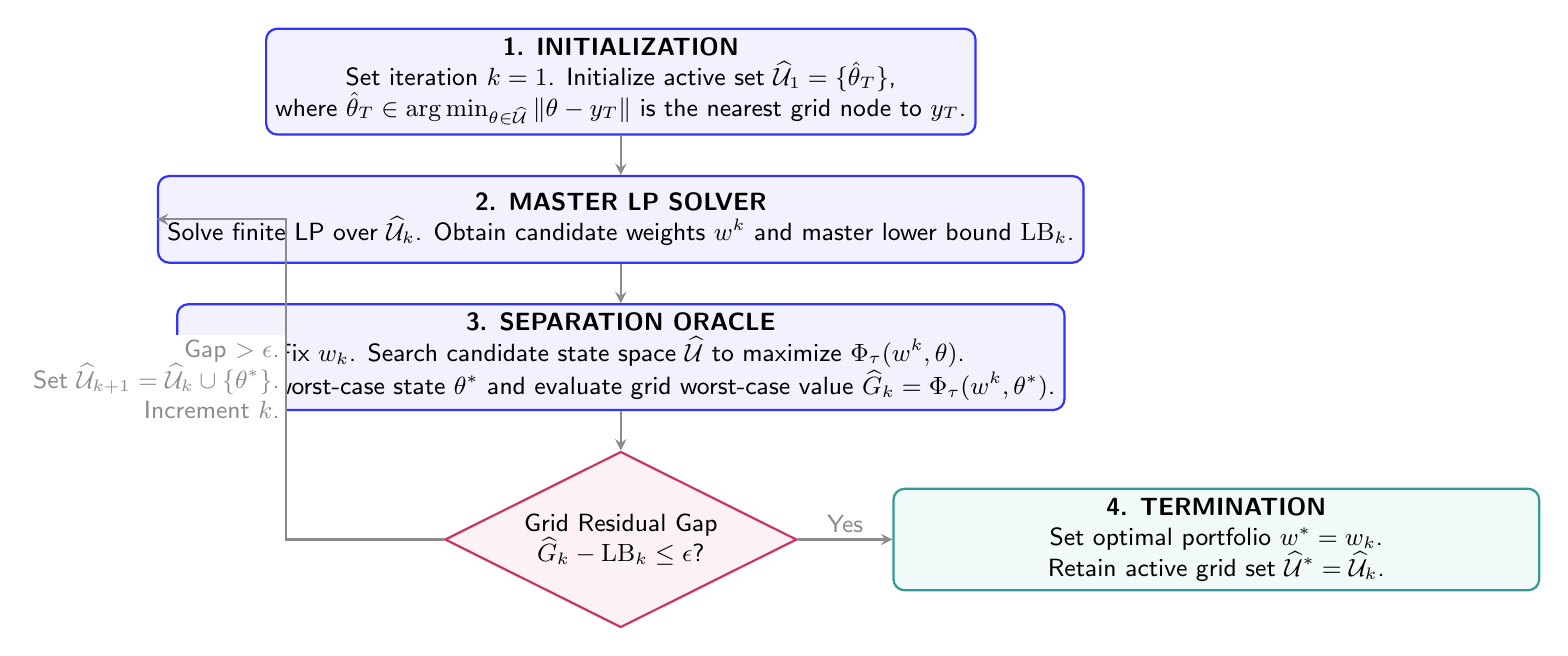
\begin{tikzpicture}[
    node distance=1.4cm, 
    every node/.style={fill=white, font=\sffamily\small}, 
    box/.style={draw=blue!80, fill=blue!5, rectangle, rounded corners, thick, minimum width=8.2cm, minimum height=1.1cm, align=center},
    arrow/.style={thick, ->, >=stealth, color=gray!90}
]
\node (step1) [box] {\textbf{1. INITIALIZATION}\\Set iteration $k=1$. Initialize active set $\widehat{\mathcal{U}}_1 = \{\hat\theta_T\}$,\\where $\hat\theta_T \in \arg\min_{\theta \in \widehat{\mathcal{U}}} \|\theta - y_T\|$ is the nearest grid node to $y_T$.};
\node (step2) [box, below=0.5cm of step1] {\textbf{2. MASTER LP SOLVER}\\Solve finite LP over $\widehat{\mathcal{U}}_k$. Obtain candidate weights $w^k$ and master lower bound $\mathrm{LB}_k$.};
\node (step3) [box, below=0.5cm of step2] {\textbf{3. SEPARATION ORACLE}\\Fix $w_k$. Search candidate state space $\widehat{\mathcal{U}}$ to maximize $\Phi_\tau(w^k, \theta)$.\\Identify worst-case state $\theta^*$ and evaluate grid worst-case value $\widehat{G}_k = \Phi_\tau(w^k, \theta^*)$.};
\node (check) [draw=purple!80, fill=purple!5, diamond, aspect=2, thick, below=0.5cm of step3, align=center] {Grid Residual Gap\\$\widehat{G}_k - \mathrm{LB}_k \le \epsilon$?};
\node (step6) [box, draw=teal!80, fill=teal!5, right=1.2cm of check] {\textbf{4. TERMINATION}\\Set optimal portfolio $w^* = w_k$.\\Retain active grid set $\widehat{\mathcal{U}}^* = \widehat{\mathcal{U}}_k$.};

\draw [arrow] (step1) -- (step2);
\draw [arrow] (step2) -- (step3);
\draw [arrow] (step3) -- (check);
\draw [arrow] (check.west) -- ++(-2.0,0) |- node[pos=0.25, left, fill=white, inner sep=2pt, align=right] {Gap $> \epsilon$.\\Set $\widehat{\mathcal{U}}_{k+1} = \widehat{\mathcal{U}}_k \cup \{\theta^*\}$.\\Increment $k$.} (step2.west);
\draw [arrow] (check.east) -- node[above, fill=white, inner sep=2pt] {Yes} (step6.west);

\end{tikzpicture}
}
\caption{Grid-restricted adaptive constraint-generation algorithm}
\label{fig:schema2}
\end{figure}

\subsection{Exact continuous separation and grid-restricted separation}
We first recall the convergence guarantee obtained under exact continuous separation and then state the scope of the finite grid-restricted implementation.

\begin{proposition}[Convergence under exact separation]
Assume that each master problem is solved to exact LP optimality and the separation oracle identifies the worst-case state $\theta^* = \arg\max_{\theta \in \mathcal{U}} \Phi_\tau(w^k, \theta)$ with exact value $G(w^k) = \Phi_\tau(w^k, \theta^*)$. Then:
\begin{enumerate}
    \item The master lower bounds form a non-decreasing sequence: $\mathrm{LB}_1 \le \mathrm{LB}_2 \le \dots \le v^\star$.
    \item The oracle values satisfy $G(w_k) \ge v^\star$ for all $k \ge 1$.
    \item For any convergence tolerance $\epsilon > 0$, the exchange algorithm terminates in a finite number of iterations with an $\epsilon$-optimal portfolio $w^k \in W$ satisfying:
    \begin{equation}
        0 \le G(w^k) - v^\star \le \epsilon, \qquad \sup_{\theta \in \mathcal{U}} \bigl[\Phi_\tau(w^k, \theta) - \mathrm{LB}_k\bigr] \le \epsilon
    \end{equation}
\end{enumerate}
\end{proposition}

\begin{proof}
Because $\widehat{\mathcal{U}}_k \subseteq \widehat{\mathcal{U}}_{k+1} \subseteq \mathcal{U}$, the feasible region of the master LP shrinks monotonically, implying $\mathrm{LB}_k \le \mathrm{LB}_{k+1} \le v^\star$. For Item 2, $G(w^k) = \sup_{\theta \in \mathcal{U}} \Phi_\tau(w^k, \theta) \ge \min_{w \in W} \sup_{\theta \in \mathcal{U}} \Phi_\tau(w, \theta) = v^\star$.

For Item 3, upon termination with $G(w^k) - \mathrm{LB}_k \le \epsilon$, we have $0 \le G(w^k) - v^\star \le G(w^k) - \mathrm{LB}_k \le \epsilon$, and the portfolio $w^k$ satisfies all finite constraints in $W$ while the epigraph pair $(w^k, \mathrm{LB}_k+\varepsilon)$ is feasible for the continuous constraint set.

To establish finite termination, suppose for contradiction that the algorithm does not terminate. Then it generates an infinite sequence of states $\{\theta_k\}_{k=1}^\infty \subset \mathcal{U}$ such that $\Phi_\tau(w^k, \theta_k) - \mathrm{LB}_k > \epsilon$ for all $k$. For any $j < k$, the constraint for $\theta_j$ was included in master problem $k$, so $\Phi_\tau(w^k, \theta_j) \le \mathrm{LB}_k$. Thus $\Phi_\tau(w^k, \theta_k) - \Phi_\tau(w^k, \theta_j) > \epsilon$. Since $\Phi_\tau$ is continuous on the compact set $W\times \mathcal{U}$, it is uniformly continuous. Hence, for every $\varepsilon>0$, there exists $\delta_\varepsilon>0$ such that $\|\theta-\theta'\|<\delta_\varepsilon \implies |\Phi_\tau(w,\theta)-\Phi_\tau(w,\theta')|<\varepsilon$ uniformly for all $w\in W$. Therefore, $\|\theta_k - \theta_j\| \ge \delta_\epsilon$ for all $j < k$. A compact metric space is totally bounded and therefore cannot contain an infinite $\delta_\epsilon$-separated sequence, which contradicts the compactness of $\mathcal{U}$ \cite{hettich1993semi, lopez2007semi}. This exact-oracle convergence is a classical consequence of standard SIP exchange methods.
\end{proof}


\begin{remark}[Monotonicity of bounds]
While the master lower bounds $\mathrm{LB}_k$ are guaranteed to be monotonically non-decreasing, the separation oracle worst-case values $\widehat{G}(w^k)$ are not guaranteed to decrease monotonically at every iteration because the portfolio $w^k$ changes. However, the best incumbent worst-case value $\overline{G}_k = \min_{1 \le j \le k} \widehat{G}(w^j)$ is monotonically non-increasing by construction.
\end{remark}

\begin{remark}[Grid-restricted separation]
When the separation oracle is evaluated over a finite candidate grid $\widehat{\mathcal{U}} \subset \mathcal{U}$, it computes
\begin{equation}
\widehat{G}(w) = \max_{\theta \in \widehat{\mathcal{U}}} \Phi_\tau(w, \theta) \le \sup_{\theta \in \mathcal{U}} \Phi_\tau(w, \theta).
\end{equation}
Since $\Phi_\tau$ is continuous on the compact set $W \times \mathcal{U}$, it is uniformly continuous. Therefore, the discrepancy between the continuous and grid-restricted objectives tends to zero as the grid dispersion radius tends to zero. Consequently, all claims of `optimal' weights and `worst-case' values in the empirical sections refer strictly to grid-restricted optimality over $\widehat{\mathcal{U}}$, unless further assessed through the heuristic continuous-domain diagnostics reported in Section \ref{sec:certification}. To ensure the algorithm operates strictly over $\widehat{\mathcal{U}}$, the active subset $\widehat{\mathcal{U}}_1$ is initialized with the nearest grid node to the most recent observation $y_T$. Section \ref{sec:certification} derives a computable bound on $L_\Phi$ and reports per-window heuristic observed gaps, and the grid-refinement sensitivity analysis reported in Section \ref{sec:sensitivity} provides a complementary assessment. Regarding initialization, re-running the 20-window sensitivity subset with three active-set initializations (nearest node to $y_T$, the grid center, a five-node spread around the unconditional mean state) yields identical terminal objectives (equal to within solver tolerance $10^{-8}$) and identical iteration counts in 20 of 20 windows, indicating robustness of the exchange path to the initial active set.


The grid-resolution statistic $\rho = \sup_{\theta \in \mathcal{U}} \min_{\hat{\theta} \in \widehat{\mathcal{U}}} \|\theta - \hat{\theta}\|$ alone is a geometric metric, not a continuous-optimality certificate. However, under standard assumptions, a conservative window-specific Lipschitz constant $L_\Phi$ for the conditional CVaR would provide the error bound:
\begin{equation}
0 \le \sup_{\theta \in \mathcal{U}} \Phi_\tau(w, \theta) - \max_{\theta \in \widehat{\mathcal{U}}} \Phi_\tau(w, \theta) \le L_\Phi \rho.
\end{equation}


\end{remark}


\subsection{Derivation of the global Lipschitz constant}\label{sec:lipschitz}

We derive a global Lipschitz constant for the function $\theta \mapsto \Phi_\tau(w, \theta)$. The conditional CVaR is given by the partial minimum:
\begin{equation}
\begin{split}
    \Phi_\tau(w, \theta) &= \min_{z \in [-M_L, M_L]} F(w, z, \theta),\\
    \text{where}\quad F(w, z, \theta) &= z + \frac{1}{\tau} \sum_{t=1}^T p_t(\theta) [\ell_t(w) - z]_+ .
\end{split}
\end{equation}
where $\ell_t(w) = -x_t^\top w$. The mapping $\theta \mapsto F(w, z, \theta)$ is smooth. However, the partial minimum $\Phi_\tau(w, \theta)$ is generally nonsmooth due to the non-uniqueness of the VaR minimizer $z^*(\theta)$ and the kink in the positive part function. By Danskin's theorem and Clarke subdifferential calculus, the subgradients of $\Phi_\tau(w, \theta)$ with respect to $\theta$ are contained in the convex hull of the gradients of $F(w, z, \theta)$ evaluated at all optimal minimizers $z \in \arg\min F(w, z, \theta)$.

The gradient of $F$ with respect to $\theta$ is:
\begin{equation}
    \nabla_\theta F(w, z, \theta) = \frac{1}{\tau} \sum_{t=1}^T \nabla_\theta p_t(\theta) [\ell_t(w) - z]_+
\end{equation}
Because any VaR minimizer $z$ lies in $[-M_L, M_L]$ and $\ell_t(w) \in [-M_L, M_L]$, the term $[\ell_t(w) - z]_+$ is uniformly bounded by $2M_L$. For Nadaraya--Watson weights with a Gaussian kernel $K_H(u) \propto \exp(-\frac{1}{2} u^\top H^{-1} u)$ one has $\nabla_\theta p_t(\theta) = p_t(\theta) H^{-1}(y_{t-1} - \bar y(\theta))$ with $\bar y(\theta) = \sum_s p_s(\theta) y_{s-1}$. Since $\bar y(\theta)$ is a convex combination of the sample states, $\|y_{t-1} - \bar y(\theta)\| \le \|y_{t-1}-\theta\| + \max_s \|y_{s-1}-\theta\| \le 2R$ with $R = \sup_{\theta, t} \|y_{t-1} - \theta\|$, and $\|H^{-1}\|_2 = 1/\lambda_{\min}(H)$, so that
\begin{equation}
    \|\nabla_\theta p_t(\theta)\| \;\le\; \frac{2R}{\lambda_{\min}(H)}\, p_t(\theta).
\end{equation}
The factor $p_t(\theta)$ is essential: it is what makes the sum over $t$ collapse, since $\sum_{t=1}^T p_t(\theta) = 1$ for every $\theta$. Summing the $T$ bounds therefore yields a constant that does not grow with the sample size:
\begin{equation}
    L_\Phi := \frac{4 R M_L}{\tau \lambda_{\min}(H)}
\end{equation}
In the numerical implementation we use the Euclidean norm on the model state
coordinates $(\log \mathrm{VIX}, D)$. Over the aligned sample these coordinates
span $[2.21, 4.42] \times [0, 0.48]$, so the largest distance between a sample
state and a point of the expanded domain is $R \approx 2.5$. The maximum
absolute daily portfolio loss is $M_L \approx 0.23$, and the plug-in bandwidth
$H = T^{-1/3}\widehat\Sigma_y$ has $\lambda_{\min}(H) \approx 5.9 \times 10^{-5}$,
the small eigenvalue reflecting the low variance of the drawdown coordinate
relative to log-VIX. With $\tau = 0.05$ these values give
$L_\Phi \approx 8 \times 10^{5}$. Combined with the grid-dispersion radius
$\rho \approx 0.03$ of the $21 \times 21$ grid, the certified bound
$L_\Phi \rho$ is several orders of magnitude larger than the objective values
themselves, and is therefore vacuous in practice. This is precisely why the
manuscript reports empirical local-search diagnostics rather than relying on
the certified bound, and why tighter region-specific Lipschitz estimates are
identified as future work.

\subsection{A posteriori gap estimation via local search}\label{sec:certification}
While the adaptive algorithm operates on the finite grid $\widehat{\mathcal{U}}$, we evaluate the approximation error over the continuous domain $\mathcal{U}$. If the minimizing VaR $z^*(\theta)$ is unique, Danskin's theorem yields the gradient with respect to $\theta$. If the minimizer is non-unique, directional derivatives or generalized derivatives must be considered. Under uniqueness, the gradient is given by:
\begin{equation}
\nabla_\theta \Phi_\tau(w,\theta) = \frac{1}{\tau}\sum_{t=1}^T \nabla_\theta p_t(\theta)\,[\ell_t(w) - z^*(\theta)]_+ ,
\end{equation}
where $\nabla_\theta p_t(\theta) = p_t(\theta) H^{-1}(y_{t-1} - \bar{y}(\theta))$ with $\bar{y}(\theta) = \sum_{s=1}^T p_s(\theta) y_{s-1}$. At nondifferentiability points, generalized directional derivatives or Clarke subgradients must be used. For bounding purposes, this permits the derivation of a computable uniform Lipschitz constant $L_\Phi := \frac{4 R M_L}{\tau \lambda_{\min}(H)}$, where $R = \sup_{\theta, t}\|y_{t-1} - \theta\|$ is the maximum state distance and $M_L$ bounds the portfolio loss. 
The grid oracle thus constitutes an inexact separation oracle with additive, one-sided inexactness $\delta \le L_\Phi \rho$. We state the consequence directly: since the master lower bounds satisfy $\mathrm{LB}_k \le v^\star$ for every $\widehat{\mathcal{U}}_k \subseteq \mathcal{U}$, and since at termination $\max_{\theta \in \widehat{\mathcal{U}}} \Phi_\tau(w^k,\theta) - \mathrm{LB}_k \le \varepsilon$, the incumbent satisfies
\begin{equation}
0 \le G(w^k) - v^\star \le \varepsilon + L_\Phi \rho .
\end{equation}
This additive-oracle propagation complements the analysis of \cite{oustry2025convex}, whose relative-gap $\delta$-oracle model (and, for their cutting-plane rate results, a strong-convexity assumption on the objective) does not directly subsume our linear master objective. We validate the analytical gradient $\nabla_\theta \Phi_\tau$ using central finite differences, confirming numerical agreement to within $10^{-7}$ precision. A direct evaluation of the conservative bound $\frac{4RM_L}{\tau\lambda_{\min}(H)}$ yields values of order $10^{2}$ to $10^{3}$, which is too loose to be practically informative. We therefore rely on a heuristic a posteriori gap estimation. Column two of Table \ref{tab:gap_verification} reports the maximum observed gradient norm over a dense $201\times201$ reference grid (which provides a local empirical gauge of the function's steepness, though not a formal global Lipschitz constant). Column five reports the empirically observed gap $\widetilde G(w^*) - \widehat G(w^*)$, where $\widetilde G(w^*)$ is the best value found by refined-grid evaluation followed by projected gradient ascent (five starts from the top grid maximizers, box-projected Armijo steps, stopping at projected gradient mapping norm $<10^{-8}$). Across all tested windows, the observed gap $\widetilde G(w^*) - \widehat G(w^*)$ is below $10^{-4}$ (column five of Table \ref{tab:gap_verification}). Because $\widetilde G$ relies on local search, it strictly lower-bounds the true continuous supremum. Therefore, the true discretization gap could theoretically exceed this observed gap. Nevertheless, the small values provide strong heuristic confidence in the practical adequacy of the $21\times21$ grid. (In the COVID-19 window, the local search improvement is identically zero because the projected gradient ascent terminated without escaping the initial grid-node maximizer.)

\begin{table}[htbp]
\centering
\caption{A posteriori gap estimation for the robust discretization}
\label{tab:gap_verification}
\resizebox{\textwidth}{!}{
\begin{tabular}{lrrrr}
\toprule
\textbf{Crisis Period} & \textbf{Max Gradient Norm} & \textbf{Grid Dispersion} & \textbf{Gradient $\times$ Dispersion} & \textbf{Local Search Improvement} \\
\midrule
1998-08 (LTCM) & 13.743 & 0.043 & 0.59 & 7.04e-04 \\
2008-10 (Lehman) & 22.105 & 0.064 & 1.41 & 6.94e-18 \\
2013-05 (Taper Tantrum) & 5.451 & 0.061 & 0.33 & 1.39e-17 \\
2020-03 (COVID-19) & 96.477 & 0.067 & 6.46 & 0 \\
2022-09 (Inflation Shock) & 13.712 & 0.067 & 0.92 & 1.39e-17 \\
\bottomrule
\end{tabular}
}
\end{table}

\subsection{Dense reference-grid validation of the discretization}
\label{sec:dense_grid}
The certified bound $L_\Phi \rho$ of Section~\ref{sec:lipschitz} is too loose
to be informative, and the local search of Table~\ref{tab:gap_verification} is
heuristic. We therefore also evaluate the separation objective directly on a
dense reference grid. Because $\theta \mapsto \Phi_\tau(w^k,\theta)$ costs
$O(T)$ per evaluation on a two-dimensional box, a $1001 \times 1001$ grid of
approximately $10^6$ candidate states is computationally routine.

Across 20 evenly spaced rolling windows, the largest excess of the dense-grid
maximum over the value returned by the $21\times21$ separation oracle is
\[
\max_k \Big[ \max_{\theta \in \widehat{\mathcal{U}}^{\,1001}} \Phi_\tau(w^k,\theta)
      - \max_{\theta \in \widehat{\mathcal{U}}^{\,21}} \Phi_\tau(w^k,\theta) \Big]
= 8.53 \times 10^{-4},
\]
that is 0.085 percentage points, against worst-case CVaR levels of
approximately 4.5\%. The discretization error of the operational grid is
therefore below 2\% in relative terms on every window tested. This remains an
empirical bound rather than a certificate, since the dense grid is itself
finite; but at $10^6$ points its dispersion radius is roughly fifty times
smaller than that of the operational grid, so it provides a far more
demanding check than the local search alone.

\section{Experimental design}\label{sec:experimental}
We evaluate the out-of-sample performance, turnover efficiency, downside capital preservation, and computational scalability of the continuous-state robust portfolio framework.

\subsection{Data and rolling-window backtesting protocol}
The empirical universe comprises the Kenneth French 30 Industry Portfolios \cite{french2026data} (value-weighted daily returns), providing broad industry-level coverage of the US equity market. Daily asset returns are aligned with:
\begin{itemize}
    \item \textbf{CBOE VIX}: Daily closing prices of the CBOE Volatility Index.
    \item \textbf{Broad Market Drawdown}: Calculated daily from the equal-weighted 30-industry composite (chosen for its heightened sensitivity to broad-based sector distress) over trailing 63-day lookback windows ($D_t \in [0, 1]$).
\end{itemize}
The aligned daily dataset spans from January 1990 to 30 June 2026, comprising 9,186 daily observations.

To clarify the chronology of the 377 rolling evaluation periods over the approximately 31.5-year span, Table \ref{tab:timeline} provides the exact backtest calendar. The first 1,260 days strictly constitute the initial training window. The first allocation is computed at the close of 27 December 1994. The terminal 9 days of the dataset are omitted to maintain equally sized 21-day compounding periods.

\begin{table}[htbp]
\centering
\caption{Exact chronological boundaries of the rolling out-of-sample backtest}
\label{tab:timeline}
\begin{tabular}{ll}
\toprule
\textbf{Chronological Marker} & \textbf{Date / Value} \\
\midrule
End of first estimation window & 27 December 1994 \\
First rebalance decision date & 27 December 1994 \\
First out-of-sample daily return date & 28 December 1994 \\
End of first 21-day holding period & 26 January 1995 \\
Last rebalance decision date & 19 May 2026 \\
Last out-of-sample return date (compounded) & 17 June 2026 \\
Number of full 21-day periods & 377 \\
Unused terminal partial period & 9 trading days (until 30 June 2026) \\
\bottomrule
\end{tabular}
\end{table}


\begin{figure}[htbp]
\centering
\resizebox{0.92\textwidth}{!}{
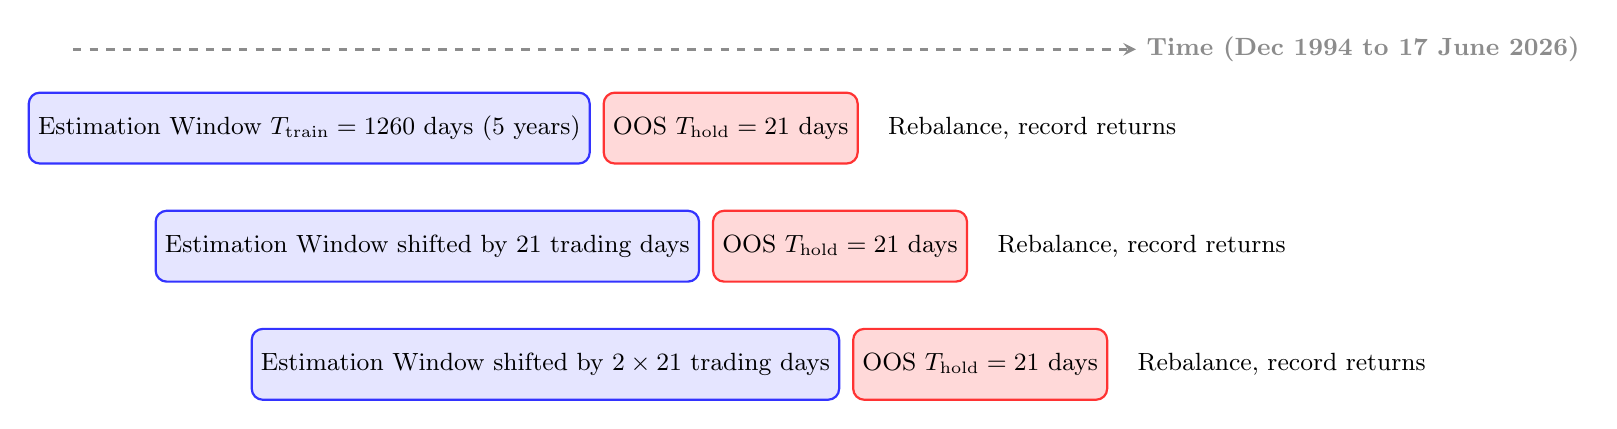
\begin{tikzpicture}[
    node distance=1cm,
    timeline/.style={draw=blue!80, fill=blue!10, thick, rounded corners, minimum height=0.9cm, font=\small},
    oos/.style={draw=red!80, fill=red!15, thick, rounded corners, minimum height=0.9cm, font=\small},
    arrow/.style={thick, ->, >=stealth, color=gray!90}
]

\node[timeline, minimum width=6cm] (train1) at (0, 2) {Estimation Window $T_{\text{train}} = 1260$ days (5 years)};
\node[oos, minimum width=1.8cm, right=0.15cm of train1] (test1) {OOS $T_{\text{hold}} = 21$ days};
\node[right=0.25cm of test1, font=\small] {Rebalance, record returns};

\node[timeline, minimum width=6cm] (train2) at (1.5, 0.5) {Estimation Window shifted by 21 trading days};
\node[oos, minimum width=1.8cm, right=0.15cm of train2] (test2) {OOS $T_{\text{hold}} = 21$ days};
\node[right=0.25cm of test2, font=\small] {Rebalance, record returns};

\node[timeline, minimum width=6cm] (train3) at (3.0, -1) {Estimation Window shifted by $2 \times 21$ trading days};
\node[oos, minimum width=1.8cm, right=0.15cm of train3] (test3) {OOS $T_{\text{hold}} = 21$ days};
\node[right=0.25cm of test3, font=\small] {Rebalance, record returns};

\draw[arrow, dashed, line width=1pt] (-3, 3) -- (10.5, 3) node[right, font=\bfseries\small] {Time (Dec 1994 to 17 June 2026)};

\end{tikzpicture}
}
\caption{The rolling-window backtesting protocol}
\label{fig:schema3}
\end{figure}

The backtest uses a rolling estimation window of $T_{\text{train}} = 1260$ trading days (approximately 5 years), as illustrated in Figure \ref{fig:schema3}. At each rebalancing date, the optimization models are estimated using only data available up to that point. The resulting allocations are held constant over the subsequent out-of-sample holding period of $T_{\text{hold}} = 21$ trading days. The backtest generates 377 consecutive 21-trading-day holding periods from 28 December 1994 to 17 June 2026.

To improve comparability across the four optimized models, the target expected return $\mu_{\text{target}}$ is dynamically set at each rebalancing date to the cross-sectional median of historical asset means: $\mu_{\text{target}} = \text{median}(\hat{\mu})$. The identical target return constraint $\hat{\mu}^\top w \ge \mu_{\text{target}}$ and weight cap $\bar{w} = 0.15$ are enforced on Robust SIP, Nominal CVaR, and Finite-Regime CVaR. In the computational implementation, $\mu_{\text{target}}$ is dynamically clamped to the attainable interval $[\mu_{\min}, \mu_{\max} - 10^{-6}]$ to guarantee strict feasibility. Over the 377 rolling out-of-sample evaluation windows, target return clamping occurred in exactly 0 periods, ensuring the original target specifications were strictly respected throughout the backtest.

We compare the continuous-state Robust SIP against four established benchmark strategies:
\begin{itemize}
    \item \textbf{1/N}: Naive equal-weighted portfolio $w_i = 1/N$.
    \item \textbf{Target-Constrained Minimum Variance (TC-MinVar)}: Minimizes portfolio variance $w^\top \widehat{\Sigma} w$ subject to $w \in W$, using the standard sample covariance matrix $\widehat{\Sigma}$. Solved via quadratic programming.
    \item \textbf{Nominal CVaR}: Minimizes unconditional historical CVaR at $95\%$ confidence level subject to $w \in W$, using uniform observation weights $1/T$.
    \item \textbf{Finite-Regime CVaR}: Minimizes the maximum CVaR across $K=4$ discrete regimes. Regimes are formed by independent median splits on log-VIX and trailing drawdown. Regime probabilities are uniform over the observations within each regime, and boundaries are recomputed in every rolling window.
\end{itemize}

To incorporate realistic market frictions, we compute holding-period portfolio turnover taking into account asset price drift over the holding period:
\begin{equation}
    \widetilde w_{i,t} = \frac{w_{i,t-1}(1+R_{i,t})}{\sum_{j=1}^N w_{j,t-1}(1+R_{j,t})}
\end{equation}
where $R_{i,t}$ is the cumulative simple/net return (and $1+R_{i,t}$ is the gross return) of asset $i$ over the 21-day holding period. Holding-period turnover and net return are defined as:
\begin{equation}
    \text{TO}_t = \frac{1}{2} \sum_{i=1}^N | w_{i,t} - \widetilde w_{i,t} |
\end{equation}
and
\begin{equation}
    r_t^{\mathrm{net}} = r_t^{\mathrm{pre-cost}} - c\,\mathrm{TO}_t,
\end{equation}
where $r_t^{\mathrm{pre-cost}}$ is the portfolio's simple holding-period return before transaction costs.

\section{Main empirical results}\label{sec:results}
\subsection{Long-term cumulative wealth and risk-adjusted performance}
Figure \ref{fig:wealth} displays the cumulative wealth trajectories of all five investment strategies net of 10 bps transaction costs on an initial \$1 investment. The naive $1/N$ portfolio delivers the highest final cumulative wealth of \$29.25, followed by the Finite-Regime CVaR portfolio (\$25.68), the continuous Robust SIP strategy (\$25.04), the Nominal CVaR portfolio (\$22.92), and the TC-MinVar portfolio (\$22.65).

\begin{figure}[H]
    \centering
    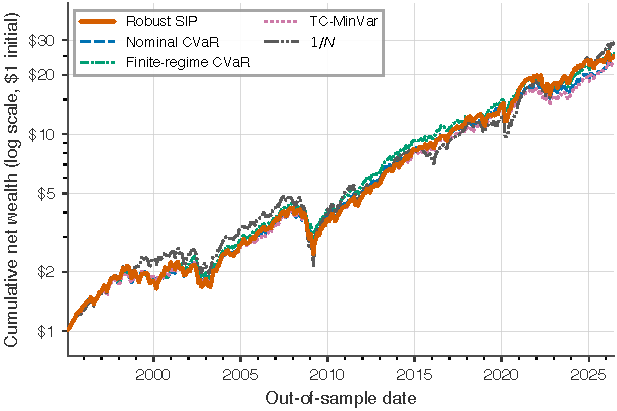
\includegraphics[width=\textwidth]{Fig1.pdf}
    \caption{Out-of-sample cumulative net wealth trajectory}
    \label{fig:wealth}
\end{figure}

\begin{table}[htbp]
\centering
\caption{Comprehensive out-of-sample performance summary (Sharpe ratios assume a zero risk-free rate)}
\label{tab:performance}
\resizebox{\textwidth}{!}{
\begin{tabular}{lrrrrr}
\toprule
\textbf{Strategy} & \textbf{Return (\%)} & \textbf{Vol (\%)} & \textbf{Sharpe} & \textbf{Max DD (\%)} & \textbf{Turnover (\%)} \\
\midrule
1/N & 12.24 & 17.00 & 0.720 & $-55.79$ & 1.69 \\
TC-MinVar & 10.73 & 12.26 & 0.875 & $-40.18$ & 5.93 \\
Nominal CVaR & 10.76 & 12.23 & 0.880 & $-35.76$ & 8.23 \\
Finite-Regime CVaR & 11.15 & 12.38 & 0.901 & $-36.76$ & 8.78 \\
Robust SIP & 11.28 & 13.95 & 0.809 & $-41.69$ & 9.48 \\
\bottomrule
\end{tabular}
}
\end{table}

Table \ref{tab:performance} reports the 5-metric performance profile. Key findings include:
\begin{enumerate}
    \item \textbf{Return Generation}: Robust SIP achieves an annualized mean return of 11.28\%, exceeding the point estimates of Nominal CVaR (10.76\%), TC-MinVar (10.73\%), and Finite-Regime CVaR (11.15\%). It ranks second overall, behind the naive $1/N$ portfolio (12.24\%). The $1/N$ portfolio benefits from broad cross-sectional diversification and full exposure to the long-run equity market risk premium over the 31-year evaluation period.
    \item \textbf{Risk-Adjusted Ratios}: Finite-Regime CVaR achieves the highest Sharpe ratio (0.901), followed by Nominal CVaR (0.880) and TC-MinVar (0.875). Robust SIP records a Sharpe ratio of 0.809. The resulting allocations exhibit higher realized volatility and greater concentration. Determining whether this arises from return targeting, state conditioning, or sparse-boundary effects requires further decomposition.
    \item \textbf{Turnover and Concentration}: Robust SIP generates the highest average holding-period turnover (9.48\%) among optimized strategies, resulting from rolling-window re-estimation of the return-state relationship. The resulting approximate transaction cost drag is 11.37 basis points per year. The effective number of assets ($N_{\text{eff}} = 7.36$) is the most concentrated, reflecting the concentrated allocations produced by worst-state CVaR minimization under the rolling state domain and return-target constraint.
\end{enumerate}

\begin{figure}[H]
    \centering
    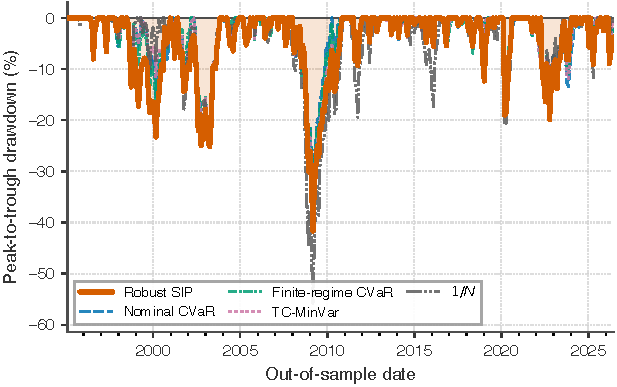
\includegraphics[width=\textwidth]{Fig2.pdf}
    \caption{Out-of-sample portfolio drawdowns over time across all strategies}
    \label{fig:drawdown}
\end{figure}

\subsection{Drawdown profiles and crisis-period performance}
Figure \ref{fig:drawdown} plots the time series of out-of-sample drawdowns. The naive $1/N$ strategy experiences severe capital destruction during major market dislocations, suffering a maximum peak-to-trough drawdown of $-55.79\%$ during the 2008 financial crisis. All optimized models experienced smaller realized maximum drawdowns than the $1/N$ portfolio over the reported sample: Nominal CVaR achieves the shallowest at $-35.76\%$, Finite-Regime CVaR reaches $-36.76\%$, and TC-MinVar reaches $-40.18\%$. Robust SIP records a maximum drawdown of $-41.70\%$, which is deeper than the unconditional CVaR benchmarks.

\begin{table}[htbp]
\centering
\caption{Crisis-period performance}
\label{tab:crisis}
\resizebox{0.88\textwidth}{!}{
\begin{tabular}{llrr}
\toprule
\textbf{Crisis Period} & \textbf{Strategy} & \textbf{Return (\%)} & \textbf{Max DD (\%)} \\
\midrule
DotCom & 1/N & $-4.75$ & $-24.41$ \\
DotCom & TC-MinVar & 1.36 & $-20.66$ \\
DotCom & Nominal CVaR & 5.86 & $-20.66$ \\
DotCom & Finite-Regime CVaR & 17.26 & $-20.33$ \\
DotCom & Robust SIP & 4.25 & $-24.95$ \\
GFC & 1/N & $-53.56$ & $-55.79$ \\
GFC & TC-MinVar & $-34.67$ & $-40.18$ \\
GFC & Nominal CVaR & $-31.13$ & $-35.76$ \\
GFC & Finite-Regime CVaR & $-30.91$ & $-36.76$ \\
GFC & Robust SIP & $-36.49$ & $-41.69$ \\
COVID & 1/N & $-20.18$ & $-20.64$ \\
COVID & TC-MinVar & $-12.25$ & $-15.29$ \\
COVID & Nominal CVaR & $-12.05$ & $-15.42$ \\
COVID & Finite-Regime CVaR & $-11.67$ & $-15.15$ \\
COVID & Robust SIP & $-17.44$ & $-18.99$ \\
Inflation & 1/N & $-6.05$ & $-17.24$ \\
Inflation & TC-MinVar & $-6.47$ & $-18.12$ \\
Inflation & Nominal CVaR & $-4.83$ & $-17.92$ \\
Inflation & Finite-Regime CVaR & $-7.66$ & $-18.88$ \\
Inflation & Robust SIP & $-8.59$ & $-19.86$ \\
\bottomrule
\end{tabular}
}
\end{table}

Table \ref{tab:crisis} presents the crisis-period analysis. During the Dot-Com crash, Finite-Regime CVaR achieved the highest cumulative return (+17.26\%), followed by Nominal CVaR (+5.86\%) and Robust SIP (+4.25\%), while $1/N$ suffered the most ($-4.75\%$). In the Global Financial Crisis, Nominal CVaR provided the best downside protection ($-31.13\%$ cumulative, $-35.76\%$ maximum drawdown), while Robust SIP experienced a deeper drawdown of $-41.69\%$. During the COVID-19 crash, all optimized models limited losses to the $-11\%$ to $-17\%$ range, with Robust SIP absorbing a larger loss ($-17.44\%$) than the unconditional benchmarks ($-12\%$). In the 2022 inflation-driven selloff, Nominal CVaR was most resilient ($-4.83\%$), while Robust SIP suffered a larger cumulative loss ($-8.59\%$). These results show that continuous-state robustification does not uniformly improve realized crisis-period performance. Rather, it reshapes the allocation profile in ways that can amplify exposure during acute market dislocations.

\begin{figure}[htbp]
    \centering
    \begin{minipage}{0.48\textwidth}
        \centering
        
\includegraphics[width=\textwidth]{Fig3.pdf}
        \caption{Robust SIP asset allocations over time}
        \label{fig:weights_rob}
    \end{minipage}
    \hfill
    \begin{minipage}{0.48\textwidth}
        \centering
        
\includegraphics[width=\textwidth]{Fig4.pdf}
        \caption{TC-MinVar asset allocations over time}
        \label{fig:weights_mv}
    \end{minipage}
\end{figure}

Figures \ref{fig:weights_rob} and \ref{fig:weights_mv} compare the dynamic allocation weights of Robust SIP and TC-MinVar. Robust SIP maintains allocations across 7 to 10 active industry sectors ($N_{\text{eff}} = 7.36$), reallocating capital across cyclical and defensive sectors as historical window dynamics evolve. Conversely, the TC-MinVar portfolio remains concentrated in low-beta industries ($N_{\text{eff}} = 8.15$), and exhibits lower realized volatility and different sector exposures.

\begin{figure}[H]
    \centering
    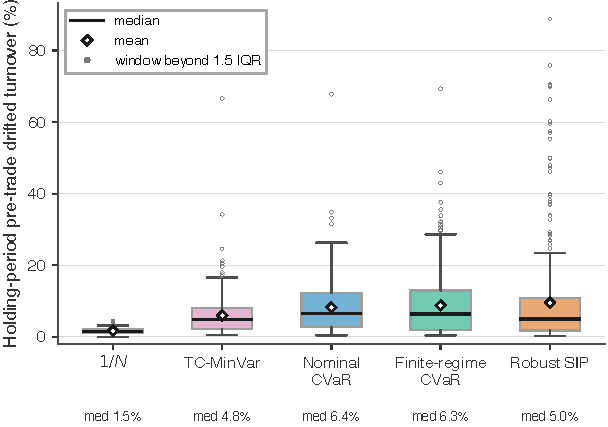
\includegraphics[width=\textwidth]{Fig5.pdf}
    \caption{Distribution of holding-period portfolio turnover}
    \label{fig:turnover}
\end{figure}

Figure \ref{fig:turnover} confirms that the turnover distribution for Robust SIP has a mean near 9.5\%, reflecting active rebalancing induced by rolling re-estimation of the return-state relationship, kernel weights, state-domain boundaries, and return target. TC-MinVar exhibits lower mean turnover (7.0\%), while $1/N$ has the lowest (1.7\%) due to its static equal-weight target. Figure \ref{fig:cumulative_tc} accumulates these per-rebalancing differences into the total transaction-cost drag borne by each strategy over the out-of-sample period.


\begin{figure}[H]
    \centering
    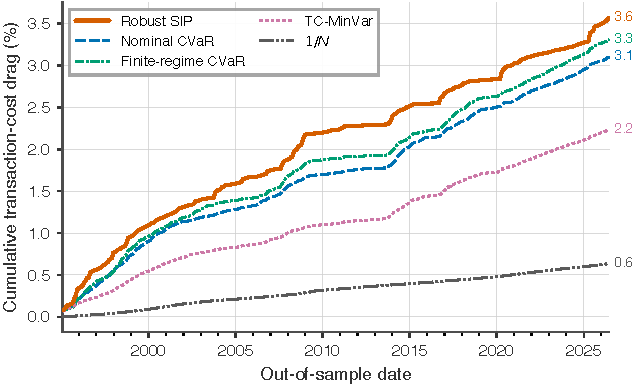
\includegraphics[width=\textwidth]{Fig6.pdf}
    \caption{Cumulative transaction cost impact}
    \label{fig:cumulative_tc}
\end{figure}


\begin{table}[htbp]
\centering
\caption{Transaction cost sensitivity: out-of-sample performance under alternative cost levels}
\label{tab:tc_sensitivity}
\resizebox{0.92\textwidth}{!}{
\begin{tabular}{lrrrrrrrrrr}
\toprule
& \multicolumn{5}{c}{\textbf{Sharpe Ratio (net of TC)}} & \multicolumn{5}{c}{\textbf{Final Wealth (\$, net of TC)}} \\
\cmidrule(lr){2-6} \cmidrule(lr){7-11}
\textbf{Strategy} & \textbf{0 bps} & \textbf{5 bps} & \textbf{10 bps} & \textbf{20 bps} & \textbf{50 bps} & \textbf{0 bps} & \textbf{5 bps} & \textbf{10 bps} & \textbf{20 bps} & \textbf{50 bps} \\
\midrule
1/N & 0.721 & 0.720 & 0.720 & 0.719 & 0.715 & 29.43 & 29.34 & 29.25 & 29.06 & 28.52 \\
TC-MinVar & 0.881 & 0.878 & 0.875 & 0.869 & 0.852 & 23.16 & 22.90 & 22.65 & 22.16 & 20.73 \\
Nominal CVaR & 0.888 & 0.884 & 0.880 & 0.872 & 0.848 & 23.63 & 23.27 & 22.92 & 22.22 & 20.26 \\
Finite-Regime CVaR & 0.909 & 0.905 & 0.901 & 0.892 & 0.867 & 26.53 & 26.10 & 25.68 & 24.85 & 22.52 \\
Robust SIP & 0.817 & 0.813 & 0.809 & 0.801 & 0.777 & 25.94 & 25.49 & 25.04 & 24.17 & 21.74 \\
\bottomrule
\end{tabular}
}
\end{table}

Table \ref{tab:tc_sensitivity} examines transaction cost sensitivity across 0, 5, 10, 20, and 50 bps. Finite-Regime CVaR records the highest point-estimate Sharpe ratio across all reported transaction-cost levels, maintaining a Sharpe ratio above 0.867 even at 50 bps. Robust SIP remains competitive in absolute wealth generation: at 50 bps, its final wealth of \$21.74 exceeds Nominal CVaR (\$20.26) and TC-MinVar (\$20.73), though it trails Finite-Regime (\$22.52). The $1/N$ portfolio is least sensitive to transaction costs due to its minimal turnover, retaining \$28.52 at 50 bps.

\section{Computational results}\label{sec:computational}
Figure \ref{fig:active_states} illustrates the number of active stress states retained by the master problem across all 377 rolling backtest windows. Across the entire 31-year backtest, the algorithm consistently converges while retaining between 1 and 9 active market states (average 3.66) out of the 441 candidate states in $\widehat{\mathcal{U}}$. Under the implemented initialization and one-state-per-iteration update rule, the reported number of active states coincides with the recorded number of master-problem solves (average 3.66 iterations).

\begin{figure}[H]
    \centering
    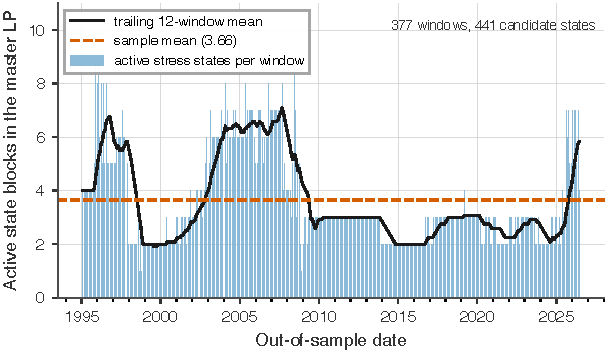
\includegraphics[width=\textwidth]{Fig7.pdf}
    \caption{Active state blocks across rolling windows}
    \label{fig:active_states}
\end{figure}

\begin{figure}[H]
    \centering
    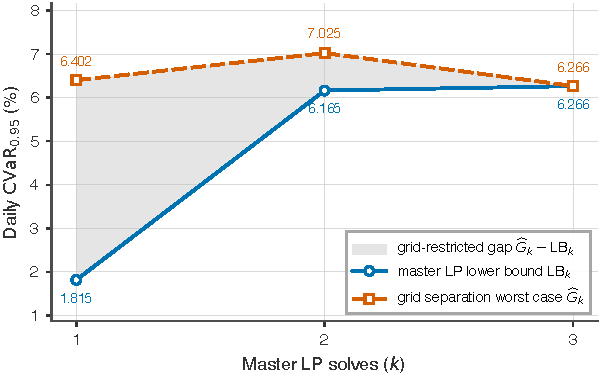
\includegraphics[width=\textwidth]{Fig8.pdf}
    \caption{Grid-restricted convergence of the lower and upper bounds}
    \label{fig:bounds}
\end{figure}

Figure \ref{fig:bounds} tracks the convergence of the Master LP Lower Bound ($\mathrm{LB}_k$) and the Grid Separation Worst-Case Value ($\widehat{G}_k$). The shaded green area denotes the grid-restricted exchange gap ($\widehat{G}_k - \mathrm{LB}_k$). Starting from an initial gap at iteration $k=1$, the oracle worst-case value fluctuates as the portfolio changes, while the master lower bound increases monotonically and the residual gap eventually closes. After 3 exchange iterations, the grid-restricted residual gap falls below $10^{-4}$, confirming numerical convergence to the finite robust problem over the $21\times 21$ candidate grid.

\begin{table}[htbp]
\centering
\caption{Computational benchmark: adaptive exchange algorithm vs. dense grid approximation}
\label{tab:computational}
\resizebox{1.0\textwidth}{!}{
\begin{tabular}{llrlr}
\toprule
\textbf{Method} & \textbf{Status} & \textbf{State blocks} & \textbf{Runtime} & \textbf{Reported value} \\
\midrule
Adaptive SIP $21\times 21$ & Exchange tolerance reached & 5 & 3.45 s & final grid worst-case CVaR $\approx$ 3.3585\% \\
Dense $21\times 21$ & OPTIMAL & 441 & 71.43 s & optimum $\approx$ 3.3578\% \\
Dense $41\times 41$ & TIME\_LIMIT / no primal solution & 1681 & 632.25 s & N/A \\
\bottomrule
\end{tabular}
}
\end{table}


\begin{table}[htbp]
\centering
\caption{Distribution of the window-level mean ESS across active stress states}
\label{tab:ess_diagnostics}
\begin{tabular}{lr}
\toprule
\textbf{Statistic} & \textbf{Value} \\
\midrule
Minimum window-level mean ESS & 2.18 \\
5th Percentile window-level mean ESS & 17.0 \\
Median window-level mean ESS & 72.8 \\
Mean window-level mean ESS & 83.0 \\
Maximum window-level mean ESS & 264.4 \\
\bottomrule
\end{tabular}
\end{table}

Figure \ref{fig:bounds} illustrates convergence for one selected rolling window. Table \ref{tab:computational} reports a single representative-window snapshot used specifically for the dense-grid benchmarking, as running the exact dense $41\times41$ LP over all 377 windows proved computationally prohibitive. Therefore, the objective values and numbers of active states in Figure \ref{fig:bounds} and Table \ref{tab:computational} are not expected to coincide. For the selected benchmark window and the reported extensive-form implementation, the dense $41\times41$ LP did not return a primal solution within the 600-second solver limit. (We note that a row-generation implementation on the dense grid would provide a more competitive alternative than the extensive-form LP.)

Several diagnostics in Tables \ref{tab:computational} and \ref{tab:ess_diagnostics} warrant careful interpretation:
\begin{enumerate}
    \item \textbf{Representative-Window $\ell_1$ Weight Discrepancy}: On the representative window, the $\ell_1$ distance between the adaptive $21\times21$ exchange solution and the dense $21\times21$ grid solution is $\|w_{\mathrm{adaptive}}-w_{\mathrm{dense21}}\|_1 \approx 0.00156$. The difference between the adaptive final grid worst-case value and the dense-grid optimum is approximately $7.6\times10^{-6}$, below the exchange tolerance of $10^{-4}$.
    \item \textbf{Active-State Support}: The minimum, across rolling windows, of the within-window mean ESS over active states is 2.18, indicating that some windows contain collectively low-support active states. The reported value $\tau\times \operatorname{ESS}$ is only a descriptive tail-support proxy and is not a formal tail effective sample size.\end{enumerate}

Figure \ref{fig:ess_history} traces the window-level mean ESS over active stress states across the 377 rolling windows, showing that the low-support episodes are concentrated in a small number of windows rather than spread uniformly over the sample.


\begin{figure}[htbp]
    \centering
    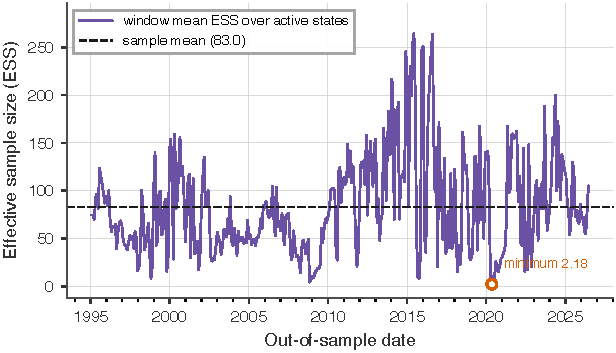
\includegraphics[width=\textwidth]{Fig9.pdf}
    \caption{Evolution of the average Effective Sample Size}
    \label{fig:ess_history}
\end{figure}


\begin{figure}[htbp]
    \centering
    \begin{minipage}{0.48\textwidth}
        \centering
        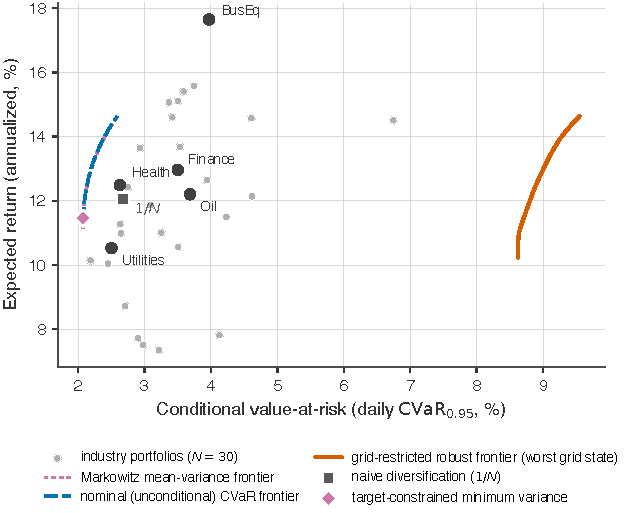
\includegraphics[width=\textwidth]{Fig10.pdf}
        \caption{In-sample risk-return efficient frontiers (15\% weight cap)}
        \label{fig:frontier}
    \end{minipage}
    \hfill
    \begin{minipage}{0.48\textwidth}
        \centering
        
\includegraphics[width=\textwidth]{Fig11.pdf}
        \caption{State density and active stress states}
        \label{fig:kernel}
    \end{minipage}
\end{figure}

Figure \ref{fig:frontier} contextualizes the in-sample decision environment. The grid-restricted robust efficient frontier forms an outer envelope of worst-grid-state CVaR values, positioned to the right of the unconditional nominal CVaR frontier and the classical Markowitz mean-variance frontier. Individual industry portfolios exhibit substantial dispersion in both expected return and downside tail risk, with defensive sectors displaying lower tail risk compared to high-beta sectors.

Figure \ref{fig:kernel} visualizes the continuous market-state space $\mathcal{U} \subset \mathbb{R}^2$ alongside the bivariate kernel density estimate $f(\text{log-VIX}, \text{Drawdown})$. Historical market states concentrate in a low-volatility, low-drawdown core regime (VIX between 10 and 20, Drawdown below 10\%). However, the continuous domain extends outward into severe tail regions, encompassing major historical dislocations such as the 1998 LTCM collapse (VIX 45.74, Drawdown 19.3\%), the 2000 to 2002 Dot-Com crash (VIX 45.08, Drawdown 44.7\%), the 2008 Lehman Brothers crisis (VIX 80.06, Drawdown 48.4\%), the March 2020 COVID-19 shock (VIX 82.69, Drawdown 33.8\%), and the 2022 inflation-driven bear market (VIX 34.02, Drawdown 24.5\%). In the representative visualization, some active stress states lie in relatively low-density regions of the state domain, exerting binding constraints on the master portfolio problem. To mitigate the computational burden and prevent over-conservatism, one could restrict the Cartesian grid $\widehat{\mathcal{U}}$ to the empirical convex hull of the observed data, thereby eliminating artificial corner states that lack any historical precedent while preserving the interpolative properties of the kernel density.

\begin{figure}[H]
    \centering
    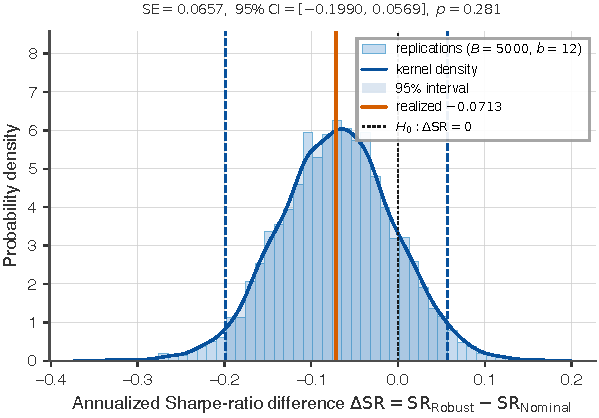
\includegraphics[width=\textwidth]{Fig12.pdf}
    \caption{Bootstrap distribution of the Sharpe-ratio difference (computed using a zero risk-free rate)}
    \label{fig:bootstrap}
\end{figure}

To rigorously assess whether the observed performance differences are statistically distinguishable from sample noise, we implement the circular block percentile bootstrap of \citet{politis1991circular} for the Sharpe-ratio difference. Because financial returns exhibit temporal dependence and volatility clustering, standard i.i.d. $t$-tests produce severely understated standard errors. This nonparametric inference provides an exploratory assessment of performance stability. We resample holding-period strategy return pairs using a block size of $b = 12$ periods over $B = 5{,}000$ bootstrap replications. Table \ref{tab:bootstrap} reports the point estimate, two-sided 95\% confidence interval, and bootstrap $p$-value for the zero-rate Sharpe ratio difference $\Delta \text{SR} = \text{SR}_{\text{Robust}} - \text{SR}_{\text{Benchmark}}$ against all four benchmarks. The bootstrap $p$-values exceed 0.13 across all benchmarks, indicating that the null hypothesis of equal Sharpe ratios cannot be rejected at conventional significance levels at the 5\% level.

\begin{table}[htbp]
\centering
\caption{Paired circular moving-block bootstrap inference for out-of-sample Sharpe ratio differences (zero risk-free rate)}
\label{tab:bootstrap}
\small
\begin{tabular}{lrrrr}
\toprule
\textbf{Benchmark} & \textbf{$\Delta$ Sharpe} & \textbf{Std Error} & \textbf{95\% CI} & \textbf{$p$-value} \\
\midrule
Nominal CVaR & -0.0713 & 0.0657 & [-0.1990, 0.0569] & 0.281 \\
1/N & 0.0890 & 0.0928 & [-0.1036, 0.2584] & 0.330 \\
TC-MinVar & -0.0663 & 0.0674 & [-0.2082, 0.0564] & 0.327 \\
Finite-Regime CVaR & -0.0919 & 0.0613 & [-0.2157, 0.0261] & 0.130 \\
\bottomrule
\end{tabular}
\end{table}

Against all four benchmarks, the bootstrap $p$-values exceed 0.05 ($p = 0.281$ vs. Nominal CVaR, $p = 0.330$ vs. $1/N$, $p = 0.327$ vs. TC-MinVar, and $p = 0.130$ vs. Finite-Regime). The bootstrap results therefore do not provide evidence against equality of the Sharpe ratios at the 5\% or 10\% significance levels. As shown in Figure \ref{fig:bootstrap}, the bootstrap distribution of $\Delta \text{SR}$ relative to Nominal CVaR is approximately symmetric and centered near the observed estimate $-0.071$. The bootstrap confidence intervals provide an exploratory gauge of estimation uncertainty, with the null value $\Delta \text{SR} = 0$ comfortably contained within the 95\% confidence interval in all four comparisons.

This statistical finding provides an important nuance to the wealth accumulation results: while Robust SIP generates competitive cumulative wealth (\$25.04 vs. \$22.92 for Nominal CVaR), its risk-adjusted Sharpe ratio is lower due to elevated portfolio volatility. The bootstrap does not provide sufficient evidence to distinguish these Sharpe-ratio differences from zero at conventional significance levels. The primary methodological contribution of the continuous-state framework lies in its principled representation of the state-risk relationship and sparse constraint generation, rather than in statistically dominant out-of-sample risk-adjusted performance.

\subsection{Reproducibility, open science, and codebase}
To ensure scientific transparency and enable independent verification of all empirical results, the entire computational framework is open-source under an MIT License. The exact code and results corresponding to this manuscript are available in the official release \cite{bezoui2026robust}.

The repository provides the complete pipeline structured into four main components:
\begin{enumerate}
    \item \textbf{Optimization Engine} (\texttt{code/RobustSIP.jl}): Implements the grid-restricted adaptive constraint-generation algorithm, the HiGHS master-LP solver, the full-grid separation oracle, and the benchmark solvers.
    \item \textbf{Backtesting Suite} (\texttt{code/main\_exp.jl}): Executes the 31-year rolling-window out-of-sample backtest, computes the 14 performance metrics, performs transaction cost sensitivity sweeps, and conducts the paired circular moving-block bootstrap test.
    \item \textbf{Empirical Data Module} (\texttt{data/aligned\_market\_data.csv}): Contains the synchronized daily returns for the Kenneth French 30 Industry Portfolios \cite{french2026data} alongside CBOE VIX and drawdown indicators over the full 1990 to 2026 period.
    \item \textbf{Figure Generation Routine} (\texttt{code/}\allowbreak\texttt{generate\_publication\_figures.py}): Reproduces all analytical figures in high-resolution vector PDF format.
\end{enumerate}

Computations were performed on an Apple M1 Pro with 8 CPU cores and 16 GB RAM, using Julia 1.11.6 \cite{bezanson2017julia}, CSV 0.10.16, DataFrames 1.8.2, JuMP 1.31.1 \cite{dunning2017jump}, and HiGHS 1.24.1 \cite{huangfu2018parallelizing} (with default presolve, tolerances at $10^{-8}$, and single-threaded execution; warm starts across exchange iterations were disabled to ensure strict benchmarking consistency). Reported solve times encompass model construction and solver execution.

\section{Model sensitivity}\label{sec:sensitivity}
To ensure the robustness of our findings to methodological hyperparameters, we conduct sensitivity analyses across key design choices: grid resolution, kernel bandwidth, Effective Sample Size (ESS) regularization, and bootstrap block length. The grid resolution and bandwidth analyses (Tables \ref{tab:sens_grid} and \ref{tab:sens_bw}) report averages over a representative subset of 20 evenly spaced rolling out-of-sample windows spanning the full evaluation period from 28 December 1994 to 17 June 2026. This uniform sampling guarantees that the analyses span multiple market regimes, including crisis periods, while remaining computationally tractable for the dense grid benchmarks. The ESS threshold and bootstrap block length sensitivities are evaluated over the entire sequence of 377 rolling windows.

\subsection{Grid resolution and bandwidth sensitivity}
Table \ref{tab:sens_grid} details the sensitivity of the adaptive exchange algorithm to the separation oracle's grid density. The standard implementation uses a $21\times21$ grid (441 candidate states). Increasing the grid resolution from $11\times11$ to $81\times81$ increases the average worst-case CVaR from approximately 4.46\% to 4.53\%, with limited objective variation beyond the $21\times21$ grid. Nevertheless, the average $\ell_1$ allocation distance between the $21\times21$ and $81\times81$ solutions is approximately 0.063, indicating that objective stability does not imply complete allocation stability. Average solve time remains below one second for all examined grids. Table \ref{tab:computational} reports one representative-window wall-clock measurement covering kernel-matrix preparation within the solver routine, JuMP model construction, and HiGHS execution. Table \ref{tab:sens_grid} reports averages over 20 rolling-window instances. The two timing experiments therefore differ in both selected instances and aggregation and should not be compared as identical benchmarks.

\begin{table}[htbp]
\centering
\caption{Grid size sensitivity: impact on solve time, active states, and objective}
\label{tab:sens_grid}
\begin{tabular}{lrrrr}
\toprule
\makecell[l]{\textbf{Grid}\\\textbf{resolution}} & \makecell[r]{\textbf{Runtime}\\\textbf{(s)}} & \makecell[r]{\textbf{Active}\\\textbf{states}} & \makecell[r]{\textbf{Worst-case}\\\textbf{CVaR$_{95}$ (\%)}} & \makecell[r]{\textbf{Dist. to}\\\textbf{base}} \\
\midrule
11$\times$11 & 0.19 & 3.20 & 4.46 & 0.1213 \\
21$\times$21 & 0.26 & 3.35 & 4.52 & 0.0627 \\
41$\times$41 & 0.51 & 3.75 & 4.53 & 0.0107 \\
81$\times$81 & 0.82 & 3.70 & 4.53 & 0.0 \\
\bottomrule
\end{tabular}
\end{table}

Table \ref{tab:sens_bw} reports sensitivity to the kernel bandwidth scalar $c \in \{0.5, 0.75, 1.0, 1.5, 2.0\}$. As bandwidth increases, the kernel density estimate becomes smoother and less sensitive to local extreme observations, leading to a reduction in the worst-case CVaR (from 4.60\% at $c=0.5$ to 4.30\% at $c=2.0$). We retain $c=1.0$ as the baseline rule-of-thumb bandwidth. The sensitivity results show that smaller bandwidths produce higher worst-case CVaR values, while larger bandwidths smooth local state effects.

\begin{table}[htbp]
\centering
\caption{Bandwidth scalar sensitivity: impact on active states and objective}
\label{tab:sens_bw}
\begin{tabular}{lrr}
\toprule
\textbf{Scalar ($c$)} & \textbf{Active States} & \textbf{In-Sample Worst-Case CVaR$_{95}$ (\%)} \\
\midrule
0.5 & 3.65 & 4.60 \\
0.75 & 3.35 & 4.56 \\
1.0 & 3.35 & 4.52 \\
1.5 & 3.45 & 4.38 \\
2.0 & 3.30 & 4.30 \\
\bottomrule
\end{tabular}
\end{table}

\subsection{ESS regularization and bootstrap block length}
To address concerns about boundary scenario overfitting in regions of the state space with low empirical support, we evaluate an ESS-thresholded uncertainty set $\mathcal{U}_{\text{supp}} = \{\theta \in \mathcal{U} : \text{ESS}(\theta) \ge E_{\min}\}$. Table \ref{tab:sens_ess} shows that enforcing $E_{\min} = 10$ filters out over half of the candidate states (retaining 172.5 out of 441) without materially altering the worst-case CVaR (4.45\%). However, requiring $E_{\min} \ge 40$ more aggressively restricts the admissible state space, which materially reduces the estimated worst-case conditional CVaR by excluding low-support boundary states (worst CVaR drops to 2.69\%).

\begin{table}[htbp]
\centering
\caption{Effective Sample Size (ESS) regularizer sensitivity}
\label{tab:sens_ess}
\begin{tabular}{lrr}
\toprule
$E_{\min}$ & \textbf{Avg Retained States} & \textbf{In-Sample Worst-Case CVaR$_{95}$ (\%)} \\
\midrule
0.0 & 441.0 & 4.45 \\
10.0 & 172.4 & 4.45 \\
20.0 & 118.8 & 3.72 \\
40.0 & 78.6 & 2.69 \\
60.0 & 61.4 & 2.52 \\
100.0 & 42.4 & 2.26 \\
\bottomrule
\end{tabular}
\end{table}



To understand whether this in-sample regularization translates to out-of-sample improvements, we run the complete rolling backtest pipeline across four selected ESS thresholds: $E_{\min} \in \{0, 10, 20, 40\}$. Table \ref{tab:ess_backtest} reports the out-of-sample performance and active state statistics for each case. While $E_{\min}=10$ successfully excludes over 60\% of the grid (retaining an average of 39.3\% of states) and excludes candidate grid states whose ESS falls below 10, the point estimates are economically similar, although no formal equality test is conducted. Aggressive regularization ($E_{\min}=40$) slightly increases the out-of-sample Sharpe ratio but exposes the portfolio to a severe maximum drawdown ($-45.94\%$). We retain $E_{\min}=0$ as the baseline primary specification and report $E_{\min}\in\{10,20,40\}$ as support-regularized sensitivity analyses.

\begin{table}[htbp]
\centering
\caption{Out-of-sample performance across ESS thresholds ($E_{\min}$)}
\label{tab:ess_backtest}
\footnotesize
\begin{adjustbox}{max width=\textwidth}
\begin{tabular}{lrrrrrrrrr}
\toprule
\makecell[l]{\textbf{Thresh-}\\\textbf{old}} & \makecell[r]{\textbf{Ret.}\\\textbf{(\%)}} & \makecell[r]{\textbf{Vol.}\\\textbf{(\%)}} & \textbf{Sharpe} & \makecell[r]{\textbf{Max DD}\\\textbf{(\%)}} & \textbf{Wealth} & \makecell[r]{\textbf{Turn.}\\\textbf{(\%)}} & \makecell[r]{\textbf{Mean}\\\textbf{ESS}} & \makecell[r]{\textbf{Min.}\\\textbf{ESS}} & \makecell[r]{\textbf{Grid ret.}\\\textbf{(\%)}} \\
\midrule
$E_{\min} = 0$ & 11.28 & 13.95 & 0.81 & $-41.69$ & 25.04 & 9.48 & 83.0 & 2.2 & 100.0 \\
$E_{\min} = 10$ & 11.04 & 13.92 & 0.79 & $-41.71$ & 23.29 & 9.64 & 86.9 & 10.0 & 39.3 \\
$E_{\min} = 20$ & 11.02 & 13.58 & 0.81 & $-40.84$ & 23.46 & 11.27 & 92.5 & 20.0 & 27.5 \\
$E_{\min} = 40$ & 10.98 & 13.26 & 0.83 & $-45.94$ & 23.53 & 13.02 & 112.6 & 40.0 & 18.3 \\
\bottomrule
\end{tabular}
\end{adjustbox}
\end{table}

Finally, Table \ref{tab:sens_block} verifies the robustness of our statistical inference to the chosen block length $b$ in the paired circular block bootstrap. Across all block lengths from 6 to 24 holding periods, the standard error remains relatively stable, and the two-sided $p$-value for the Sharpe ratio difference against the Nominal CVaR benchmark never falls below the conventional 0.05 threshold, supporting the qualitative conclusion that the inference is not sensitive to the reported range of block lengths. The block-length sensitivity results use the same methodology as the primary bootstrap analysis. Remaining numerical differences across block lengths reflect both the altered dependence structure induced by the block length and Monte Carlo variability.

\begin{table}[htbp]
\centering
\caption{Bootstrap block length sensitivity on inference}
\label{tab:sens_block}
\begin{tabular}{rrr}
\toprule
\makecell[r]{\textbf{Block length $b$}\\\textbf{(21-day holding periods)}} & \textbf{Bootstrap SE} & \textbf{$p$-value} \\
\midrule
6 & 0.0655 & 0.270 \\
9 & 0.0658 & 0.275 \\
12 & 0.0657 & 0.281 \\
18 & 0.0618 & 0.243 \\
24 & 0.0535 & 0.183 \\
\bottomrule
\end{tabular}
\end{table}


\subsection{Support restriction and state conditioning}
\label{sec:referee_benchmarks}
Two further specifications isolate the roles of the support of the state domain
and of the robust layer itself. Both are computed on the identical 377-window
calendar and with the identical estimation window, weight cap, return target,
bandwidth rule and transaction-cost convention as the baseline, so the only
differences are the ones under study.

The first restricts the separation set to the empirical convex hull of the
training states, so that the worst case is taken only over combinations of
log-VIX and drawdown that the sample actually exhibits. Figure
\ref{fig:hull} shows the geometry for a representative window: the hull excludes
the low-volatility/high-drawdown and high-volatility/low-drawdown corners
entirely, and on average only 32.2\% of the 441 candidate states survive. The
second removes the robust layer and solves nominal CVaR under the
kernel-weighted conditional distribution at the current state $y_T$, which is
the prescriptive counterpart in the spirit of \citet{bertsimas2020predictive}.

\begin{table}[htbp]
\centering
\caption{Support-restricted and state-conditioned specifications, on the same
377-window calendar as Table \ref{tab:performance}}
\label{tab:referee_benchmarks}
\small
\begin{tabular}{lrrrrr}
\toprule
\textbf{Specification} & \makecell[r]{\textbf{Ret.}\\\textbf{(\%)}} & \makecell[r]{\textbf{Vol.}\\\textbf{(\%)}} & \textbf{Sharpe} & \makecell[r]{\textbf{Turn.}\\\textbf{(\%)}} & \textbf{Wealth} \\
\midrule
Robust SIP (baseline) & 11.28 & 13.95 & 0.809 & 9.48 & 25.04 \\
Robust SIP, hull-restricted & 11.06 & 13.99 & 0.790 & 9.47 & 23.32 \\
State-conditioned CVaR & 10.05 & 13.01 & 0.773 & 35.74 & 17.82 \\
\bottomrule
\end{tabular}
\end{table}

Table \ref{tab:referee_benchmarks} reports both. Neither variant improves on the baseline. Restricting the domain to the
empirical hull leaves the maximum drawdown and the turnover essentially
unchanged and lowers the Sharpe ratio slightly, from 0.809 to 0.790. The
low-support boundary states are therefore not the source of the risk-adjusted
shortfall documented in Section \ref{sec:results}: removing them costs a little
performance rather than recovering any. This is a useful negative result, since
it separates the support question from the performance question.

The state-conditioned specification is the more informative comparison. It is
dominated on every dimension reported here, with the lowest Sharpe ratio
(0.773), the lowest terminal wealth (\$17.82) and an average turnover of
35.7\%, nearly four times that of the baseline. Conditioning the distribution on
the single currently observed state makes the allocation track short-lived
movements in the state variables, which is precisely the instability that taking
the worst case over a state domain suppresses. Figure \ref{fig:referee_wealth}
shows the resulting wealth paths. The robust layer therefore earns its place not
by beating unconditional benchmarks on risk-adjusted terms, which it does not,
but by stabilizing an allocation that pure conditioning renders excessively
turnover-intensive.

\begin{figure}[htbp]
    \centering
    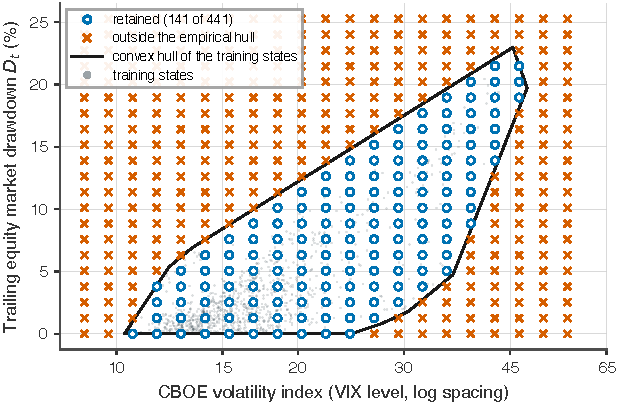
\includegraphics[width=\textwidth]{Fig14.pdf}
    \caption{Candidate states retained after restriction to the empirical convex
    hull of the training sample, for a representative rolling window. Circles
    mark retained states, crosses those excluded, and the solid line is the hull
    boundary}
    \label{fig:hull}
\end{figure}

\begin{figure}[htbp]
    \centering
    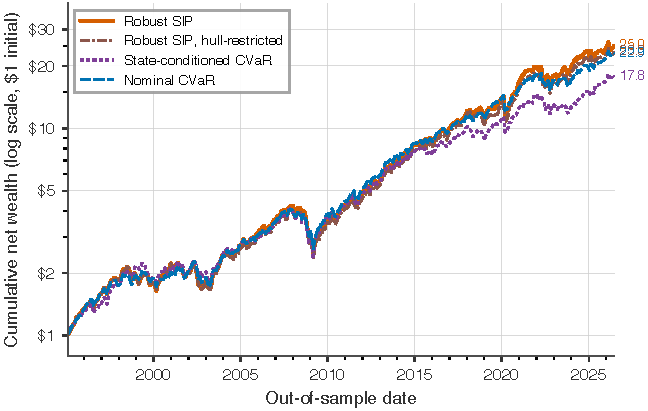
\includegraphics[width=\textwidth]{Fig13.pdf}
    \caption{Cumulative out-of-sample wealth of the support-restricted and
    state-conditioned specifications against the baseline and the strongest
    unconditional benchmark, net of 10 basis points per unit of turnover}
    \label{fig:referee_wealth}
\end{figure}

\subsection{Allocation instability and turnover constraints}
A notable property of the continuous-state robust formulation is the near-flatness of the worst-case objective surface around the optimum. Because multiple asset combinations can achieve nearly identical worst-case CVaR, the optimal allocation $w^*$ may exhibit instability across adjacent rolling windows. The grid-refinement analysis of Table \ref{tab:sens_grid} provides indirect evidence of this flatness: refining the separation grid from $21\times21$ to $81\times81$ changes the worst-case CVaR by less than $0.02$ percentage points while displacing the optimal allocation by $\|w_{21}-w_{81}\|_1 \approx 0.063$. Objective stability therefore coexists with non-trivial allocation instability, which is consistent with the elevated mean holding-period turnover of 9.48\% (median 5.0\%) reported in Table \ref{tab:performance} (11.37 bps approximate annual transaction-cost drag). While the focus of this paper is unconstrained risk minimization, practical implementations could penalize this instability, for instance by incorporating an $\ell_1$ proximity regularizer $\lambda \|w - w_{\mathrm{prev}}\|_1$ into the master LP.


\section{Discussion and conclusion}\label{sec:conclusion}
The proposed state-robust CVaR framework provides a principled and interpretable method for incorporating continuous market covariates into portfolio optimization without imposing artificial discrete regime boundaries. In the reported approximately 31.5-year empirical experiment on US industry portfolios, the continuous-state strategy achieved greater terminal wealth (\$25.04) than TC-MinVar (\$22.65) and nominal CVaR (\$22.92), but lower wealth than naive $1/N$ (\$29.25) and finite-regime CVaR (\$25.68). It also exhibited lower Sharpe ratios and deeper maximum drawdowns than the nominal and finite-regime CVaR benchmarks, and paired circular block percentile bootstrap testing does not provide sufficient evidence to distinguish these Sharpe-ratio differences from zero at conventional significance levels. Thus, the empirical findings do not establish superior risk-adjusted or crisis performance.

The principal contribution of this work is methodological and computational: a kernel-weighted family of conditional return distributions indexed by continuous financial indicators can be incorporated into a continuous-state robust optimization model whose finite grid-restricted approximation can be solved efficiently through adaptive constraint generation. Because the operational implementation uses finite-grid separation ($21\times21 = 441$ states), its numerical convergence guarantees apply directly to the grid-restricted robust problem, achieving approximately a $20.7\times$ speedup $71.43/3.45\approx20.70$ on the representative benchmark window (single-threaded HiGHS 1.24.1 \cite{huangfu2018parallelizing}, tolerance $10^{-4}$) over dense LP discretization while retaining an average of only 3.66 active state blocks (range 1-9 across 377 windows) (and requiring an average of 3.66 exchange iterations under the implementation's counting convention).

Several methodological considerations and future extensions warrant discussion. First, while the two-dimensional state space (log-VIX and drawdown) remains computationally tractable, kernel density estimation and Cartesian grid search deteriorate rapidly as state dimension increases ($M \ge 3$). Future research should explore dimension-reduction techniques, such as autoencoder latent spaces or conditional generative models, to scale continuous-state robustification. Second, in two dimensions, global grid evaluation provides an efficient separation oracle, whereas in higher dimensions, certified global branch-and-bound or interval arithmetic could provide certified continuous optimality bounds. Third, our empirical tracking of Effective Sample Size revealed that the minimum, across rolling windows, of the within-window mean ESS over active states is 2.18, indicating that some windows contain collectively low-support active stress states. Incorporating explicit ESS-thresholded uncertainty domains $\mathcal{U}_{\text{supp}} = \{\theta \in \mathcal{U} : \text{ESS}(\theta) \ge E_{\min}\}$ represents a natural regularizer to prevent boundary scenario overfitting. Fourth, integrating explicit turnover regularization directly into the master LP would further suppress transaction costs in higher-friction market environments. The framework combines non-parametric conditional risk estimation with a continuous-state semi-infinite formulation, while the empirical implementation solves a finite grid-restricted approximation efficiently through adaptive constraint generation.

\newpage


\bibliographystyle{plainnat}

\section*{Statements and Declarations}

\textbf{Funding:} The authors declare that no funds, grants, or other support were received during the preparation of this manuscript.

\textbf{Competing Interests:} The authors have no relevant financial or non-financial interests to disclose.

\textbf{Data Availability:} The Kenneth French 30 Industry Portfolio returns \cite{french2026data} and CBOE VIX observations \cite{cboe2026vix} used in this study were obtained from their publicly accessible source pages. Source URLs, retrieval information, preprocessing code, and the aligned research dataset are documented in the accompanying repository, subject to the original providers' terms of use. All reported results correspond to Zenodo version DOI 10.5281/zenodo.22309074, archived from Git commit 416b0a339040178906642df61a94c25910c11e99. The GitHub repository may contain later development versions \cite{bezoui2026robust}.

\textbf{Author Contributions:} Madani Bezoui: Conceptualization, Methodology, Software, Writing - original draft. Thiziri Sifaoui: Formal analysis, Validation, Writing - review and editing. Ahcene Bounceur: Supervision, Writing - review and editing.

\bibliography{references}


\end{document}
